
\documentclass[journal]{IEEEtran}
%%
%% Packages required after switching from acmart to IEEEtran.
\usepackage{graphicx}
\graphicspath{{figures/}{./}}
\usepackage{amsmath}
\usepackage{amssymb}
\usepackage{cite}
\usepackage[utf8]{inputenc}
\usepackage{url}
\usepackage[T1]{fontenc}
\usepackage{xcolor}
\usepackage{tikz}
\usetikzlibrary{arrows.meta,positioning,calc,fit,backgrounds}
\usepackage{booktabs}
\usepackage{tabularx}
\usepackage{makecell}
%% === ADDED: change-tracking markup (red strikethrough = deleted, green = added) ===
\usepackage[normalem]{ulem}
\definecolor{trackadd}{rgb}{0,0.55,0}
\DeclareRobustCommand{\cadd}[1]{\textcolor{trackadd}{#1}}
\DeclareRobustCommand{\cdel}[1]{\textcolor{red}{\sout{#1}}}
%% \Description is an acmart-only macro; make it a no-op under IEEEtran.
\providecommand{\Description}[1]{}

\begin{document}

\title{Spatiotemporal Deep Learning for Digital Health: From Predictive Models to Digital Twins and World Models}

\author{Xin~Xiang,~Hua~Fang,~D.~Liu,~and~Honggang~Wang%
\thanks{The authors are with the Graduate Computer Science and Engineering Department, Katz School of Health and Science, Yeshiva University, New York, NY 10016 USA (e-mail: xxiang@mail.yu.edu; julia.fang@yu.edu; dliu6@mail.yu.edu; honggang.wang@yu.edu).}}
%%
%% Sometimes the addresses are too long to fit on the page.  In this
%% case uncomment the lines below and fill them accodingly.
%%
%% \authorsaddresses{Corresponding author: Ben Trovato,
%% \href{mailto:trovato@corporation.com}{trovato@corporation.com};
%% Institute for Clarity in Documentation, P.O. Box 1212, Dublin,
%% Ohio, USA, 43017-6221}
%%
%%
%% Keywords. The author(s) should pick words that accurately describe
%% the work being presented. Separate the keywords with commas.

\maketitle

\begin{abstract}
Human health and disease progression are closely influenced by environmental, behavioral, and spatial factors. However, existing digital health research has largely relied on traditional clinical records, which lack continuous spatiotemporal context and fail to capture environmental and lifestyle exposures. While recent advances in wearable sensing and mobile health technologies enable the collection of rich longitudinal data, existing surveys typically focus on either temporal modeling or isolated data modalities, lacking a unified perspective on spatiotemporal learning in digital health. In this survey, we review recent developments in spatiotemporal modeling for digital health, covering sequence based models, graph based approaches, world model and emerging digital twin frameworks applied to longitudinal health data, environmental exposure, and lifestyle factors such as diet. We categorize existing methods, analyze their design trade-offs, and compare their applicability across different healthcare scenarios. A central theme of our review is that spatiotemporal deep learning supplies the predictive backbone for two increasingly important paradigms: world models, which learn the latent dynamics of a patient's state to support simulation and counterfactual reasoning over candidate interventions, and digital twins, which embed these learned dynamics in a continuously updated virtual representation of an individual. We show how the same spatiotemporal representations that drive health trajectory prediction also enable world models to anticipate how a patient would respond to alternative actions and allow digital twins to keep that simulation synchronized with streaming real world observations. Across the studies we survey, integrating spatial and environmental context often improves chronic disease prediction and health trajectory modeling, whereas lifestyle factors remain underused and their predictive value, though promising, is not yet systematically quantified. We further identify key challenges, including data sparsity, heterogeneity, and continuous model updating. These findings highlight the importance of developing continuous, adaptive, and personalized health modeling systems, and suggest that future research could focus on real time data integration, world model based and digital twin driven simulation, and privacy preserving learning for scalable healthcare applications.
\end{abstract}

\begin{IEEEkeywords}
Spatiotemporal models, deep neural networks, digital health, Internet of Things, wearable sensing, longitudinal data, federated learning, digital twin, world models, chronic disease.
\end{IEEEkeywords}

% \begin{figure*}[t]
%     \centering
%     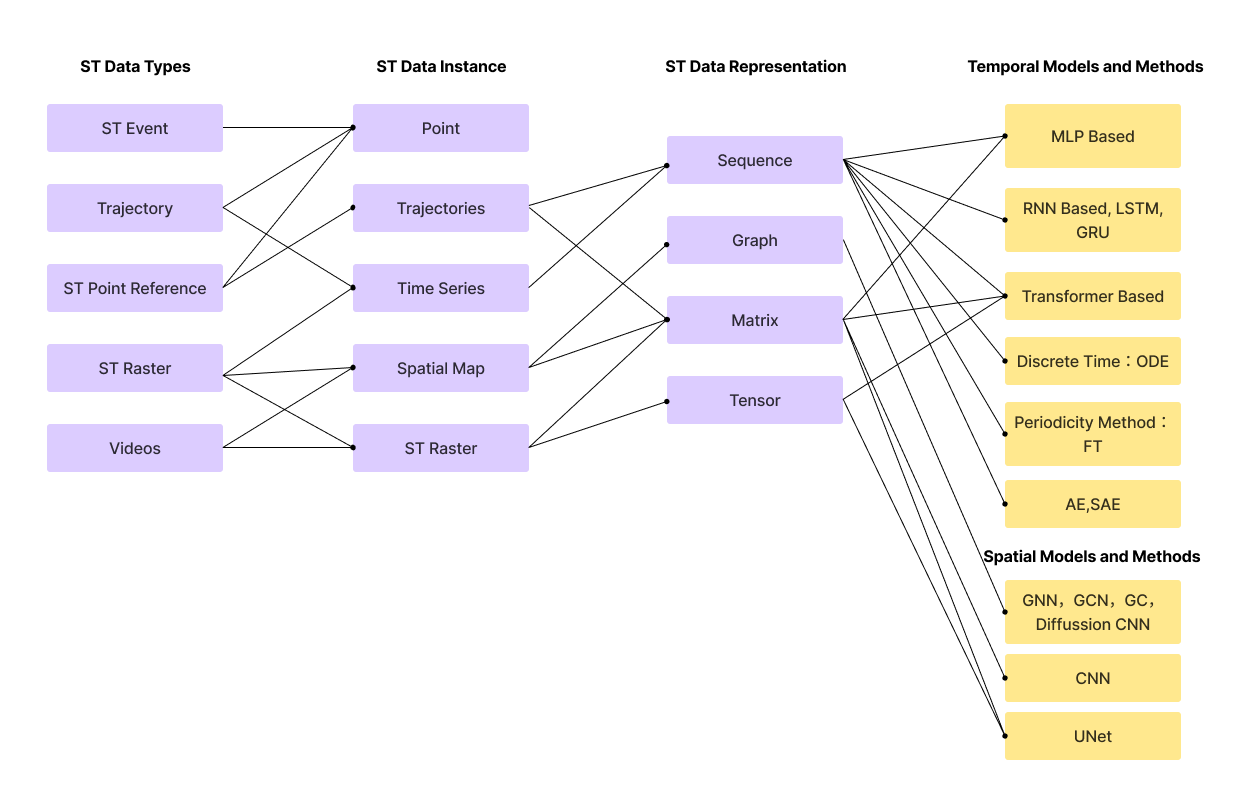
\includegraphics[width=\linewidth]{Frame 9 (3).png}
%     \caption{ST Data Categories}
%     \Description{A diagram illustrating different categories of Spatiotemporaldata (e.g., spatial only, temporal only, Spatiotemporal).}

%     \label{fig:ST Data Categories}
% \end{figure}


\section{Introduction}
Clinical decisions combine static patient characteristics, snapshot observations, and longitudinal history such as prior diagnoses, laboratory trends, and treatment responses. For chronic or progressive diseases, periodic follow up visits yield only an intermittently sampled view of health evolution that is coarse, fragmented, and disconnected from daily behavior and environmental exposure. Digital health reframes this workflow as time stamped, context dependent observations, allowing symptoms, physiological signals, behavior, and exposures to be recorded continuously and modeled as evolving trajectories.

Computational health modeling has moved from static risk estimation toward dynamic, contextual prediction. Early rule based systems were interpretable but brittle; electronic health records later enabled probabilistic and survival models, while machine learning improved nonlinear pattern recognition yet often reduced longitudinal history to aggregated features. The key shift came when temporal models represented disease evolution directly from sequential observations, accelerated by wearable sensors and mobile health. In diabetes management, for instance, models trained on continuous glucose monitoring capture short term glucose dynamics and longer term changes in insulin sensitivity, supporting responsive prediction and treatment adjustment \cite{Vaughan2025CGMPrediction,Gecili2020CGMPrediction}.

Temporal modeling alone cannot capture how health unfolds in real life. Health evolves jointly in time and space: location, food environments, air quality, physical activity, mobility, work routines, and socioeconomic context all shape physiological and behavioral trajectories. Large scale nutrition studies, for example, show that diet quality and chronic disease risk vary systematically across regions and socioeconomic groups \cite{McCullough2022Diet}. Incorporating spatial context therefore links environmental and lifestyle factors to longitudinal patient states, improving personalization and helping explain why similar clinical profiles can follow different trajectories.


\begin{figure*}
    \centering
    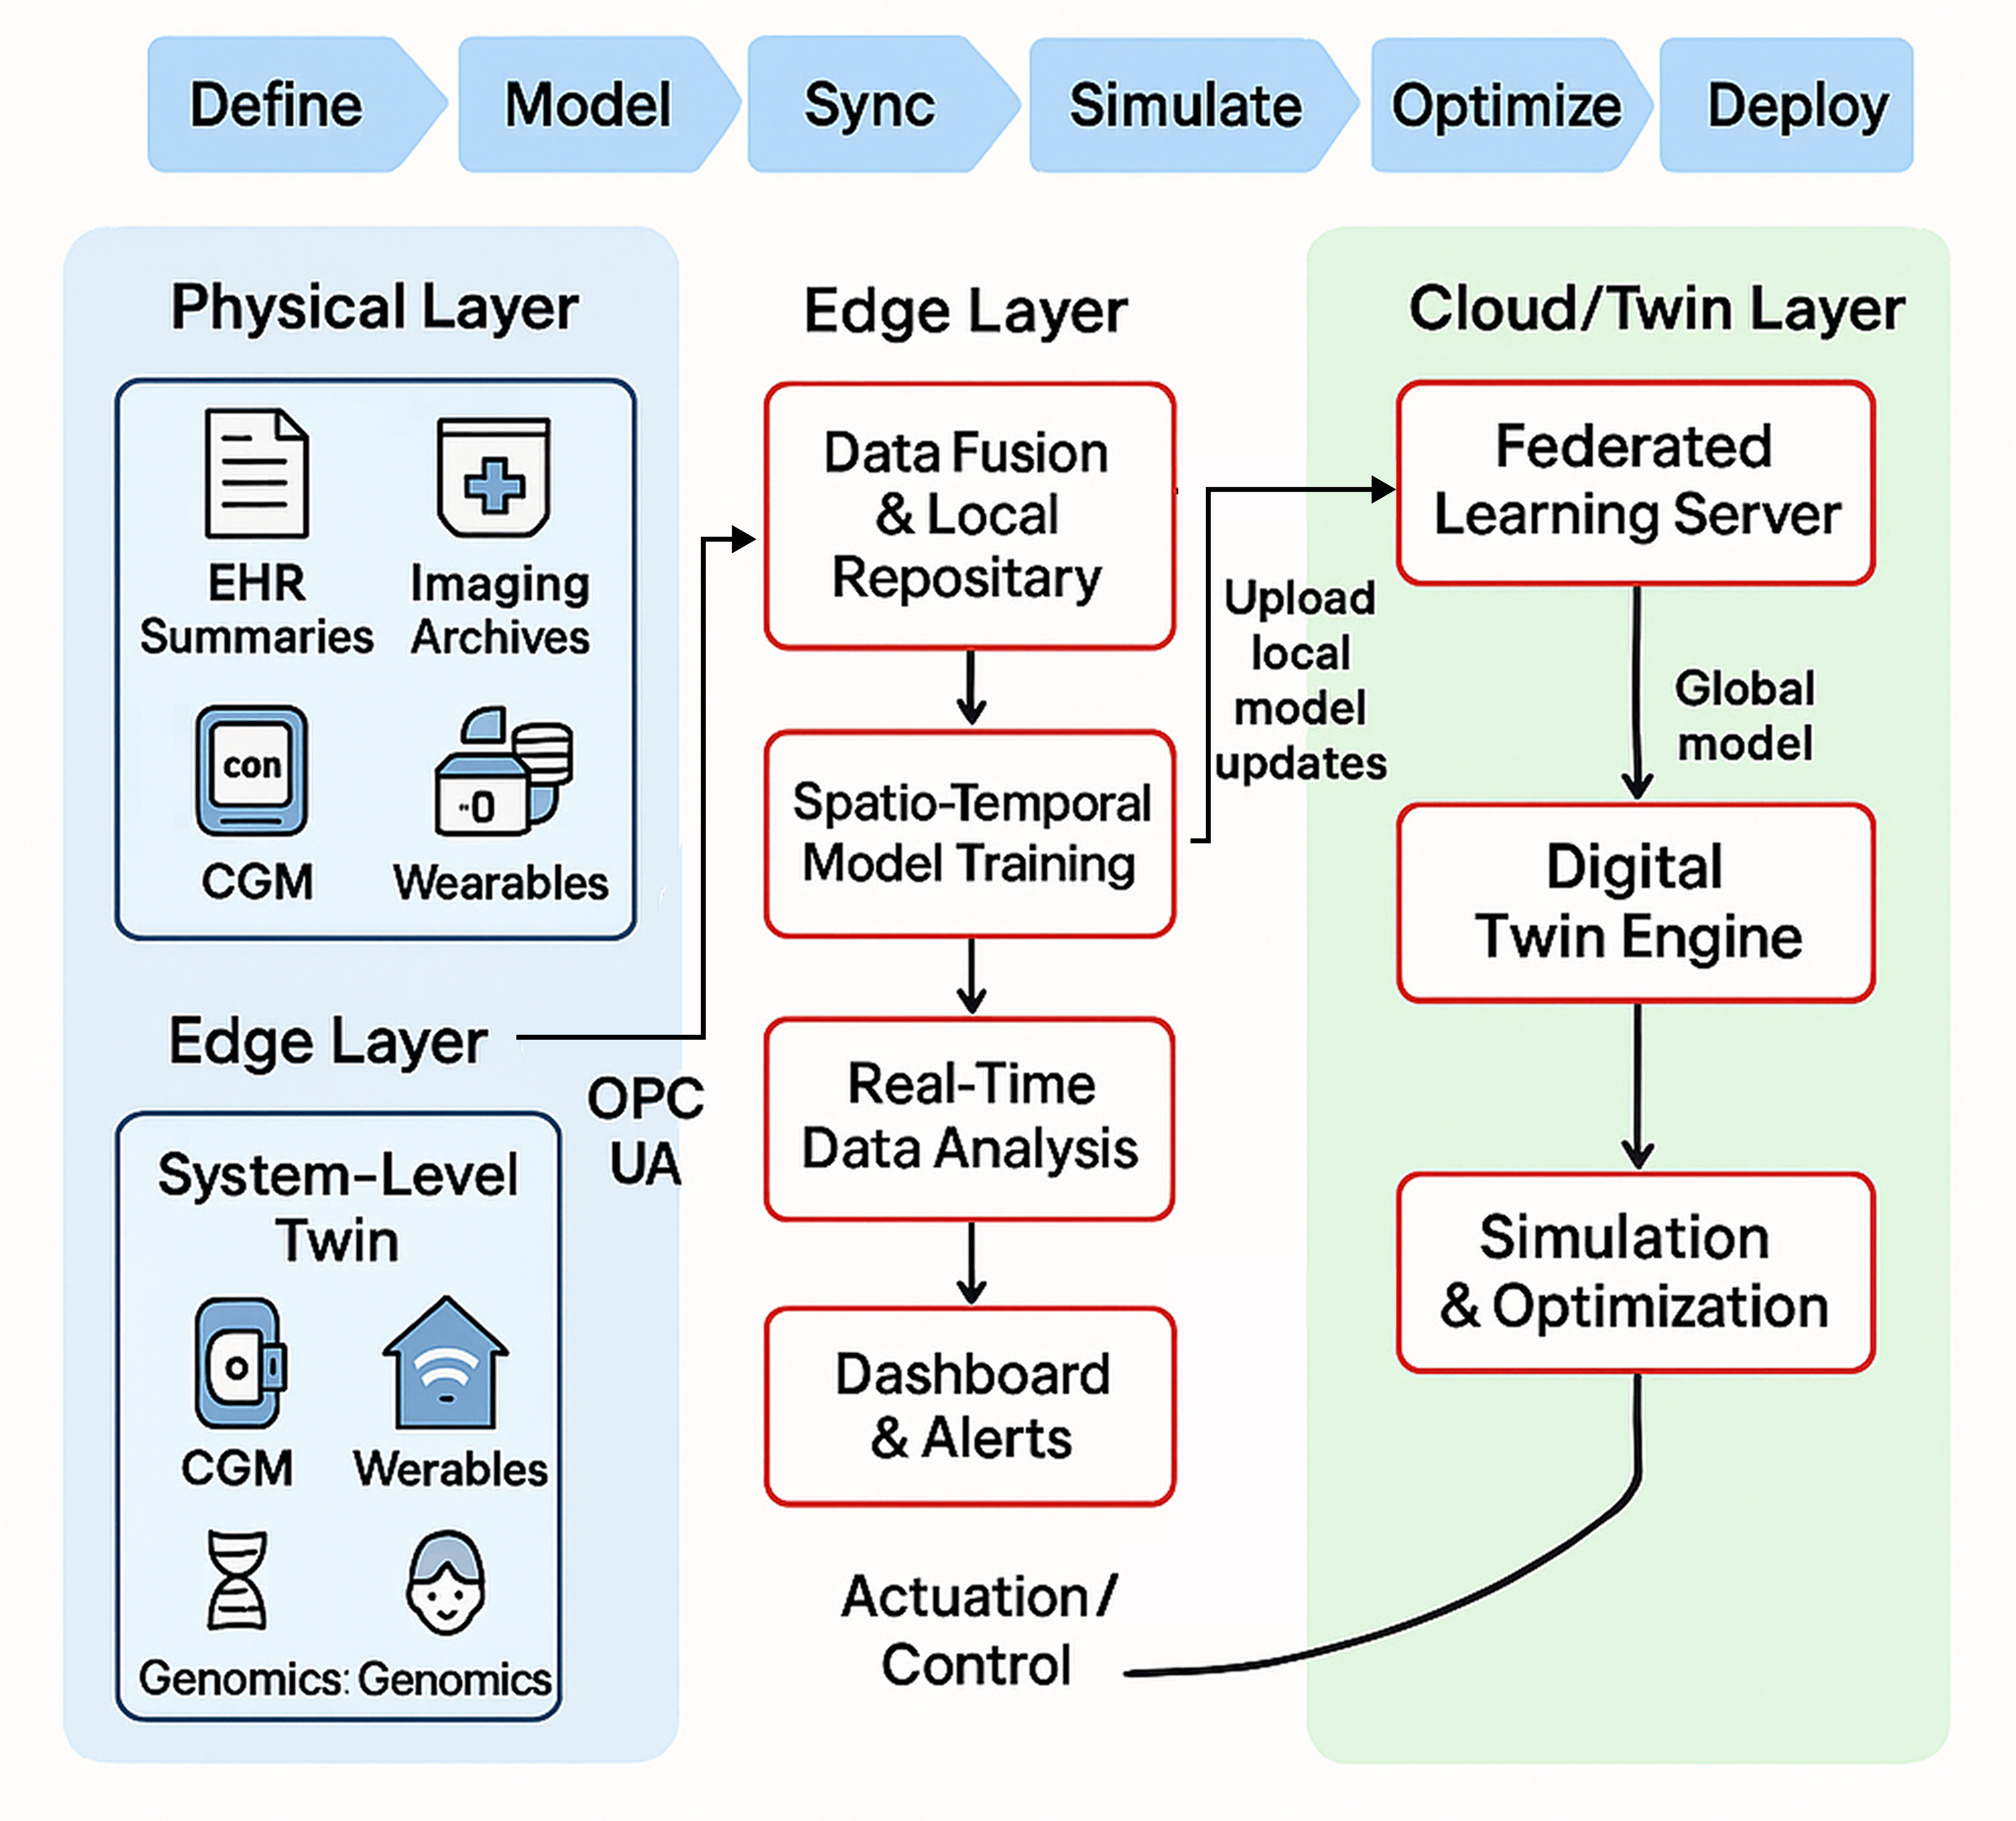
\includegraphics[width=0.6\linewidth]{digital twin in health care.png}
    \caption{Conceptual overview of a digital twin in healthcare: real world patient data from sensors, wearables, and clinical records continuously update a virtual patient replica, which supports monitoring, prediction, and intervention planning in a closed feedback loop.}
    \Description{A conceptual diagram of a digital twin in healthcare, in which real-world patient data from sensors, wearables, and clinical records continuously update a virtual patient replica that supports monitoring, prediction, and intervention planning.}
    \label{fig:digital twin in health care}
\end{figure*}
This survey argues that spatiotemporal modeling is a necessary step in this progression. Reviewing spatiotemporal models and their digital health applications, we clarify how environmental and lifestyle factors such as diet can enter longitudinal disease prediction, and how such models support faithful, personalized digital twins for healthcare.


Our audience is twofold: developers who build spatiotemporal models and researchers who deploy them in digital health or digital twin settings. We introduce a practical taxonomy, examine application scenarios, recommend data processing pipelines and model choices, and give evaluation guidance. We then address deployment privacy concerns and solutions such as federated learning, and forecast future trends in digital twin based digital health. This is a narrative survey: we draw on peer-reviewed work from IEEE Xplore, PubMed, and Scopus together with recent preprints spanning roughly 2015--2026, prioritizing methods relevant to spatiotemporal deep learning in digital health. Unlike earlier spatiotemporal data mining surveys~\cite{wang2022deep,atluri2018stdm}, which target generic domains such as traffic and climate, we focus on digital health and on the emerging link between spatiotemporal learning, world models, and digital twins.

\textbf{Our main contributions are as follows.} First, we develop a digital health taxonomy linking spatiotemporal data types (event, trajectory, point reference, raster, video), their preprocessing challenges (sparsity, irregular sampling, multi scale structure), the foundational architectures (CNN, GNN, RNN, Transformer), and clinical applications into a unified map from data to model to deployment. Second, we synthesize the major model families (CNN--RNN hybrids, spatiotemporal graph neural networks, Transformer based models, 3D-CNN and hybrid networks, and irregular time, longitudinal, and statistical deep learning approaches) with guidance on when each suits digital health data, illustrated across dietary, diabetes, depression, and cardiac applications. Third, we analyze deployment through medical digital twins, including privacy preserving federated learning, visualization, uncertainty quantification, and world model based patient simulators for counterfactual planning. Finally, we distill practical guidance on data processing, model selection, and evaluation for spatiotemporal digital health, and identify open challenges on the path to world model based digital twins.

The remainder is organized as follows. Section~\ref{sec:data} characterizes spatiotemporal data in digital health and its challenges (sparsity, irregular sampling, multi scale structure). Section~\ref{sec:history} reviews the development of deep learning based spatiotemporal methods. Section~\ref{sec:models} presents spatiotemporal models and their digital health applications across domains. Section~\ref{sec:categorization} categorizes deep learning based medical and longitudinal models. Section~\ref{sec:DT} covers integration within digital twin systems, including data collection and privacy. Section~\ref{sec:world_model_dt} develops world model based digital twins for patient state simulation and counterfactual planning. Section~\ref{sec:future} outlines future directions combining spatiotemporal modeling with digital twins.


\section{Spatiotemporal Data in Digital Health}
\label{sec:data}

Most patient related phenomena are indexed by both time and space and can be represented in four dimensions (three spatial, one temporal). Following prior work~\cite{wang2022deep,atluri2018stdm}, spatiotemporal data in digital health fall into five types---event, trajectory, point reference, raster, and video data---illustrated in Figure~\ref{fig:Five Spatio temporal Data Categories}.




\begin{figure*}
    \centering
    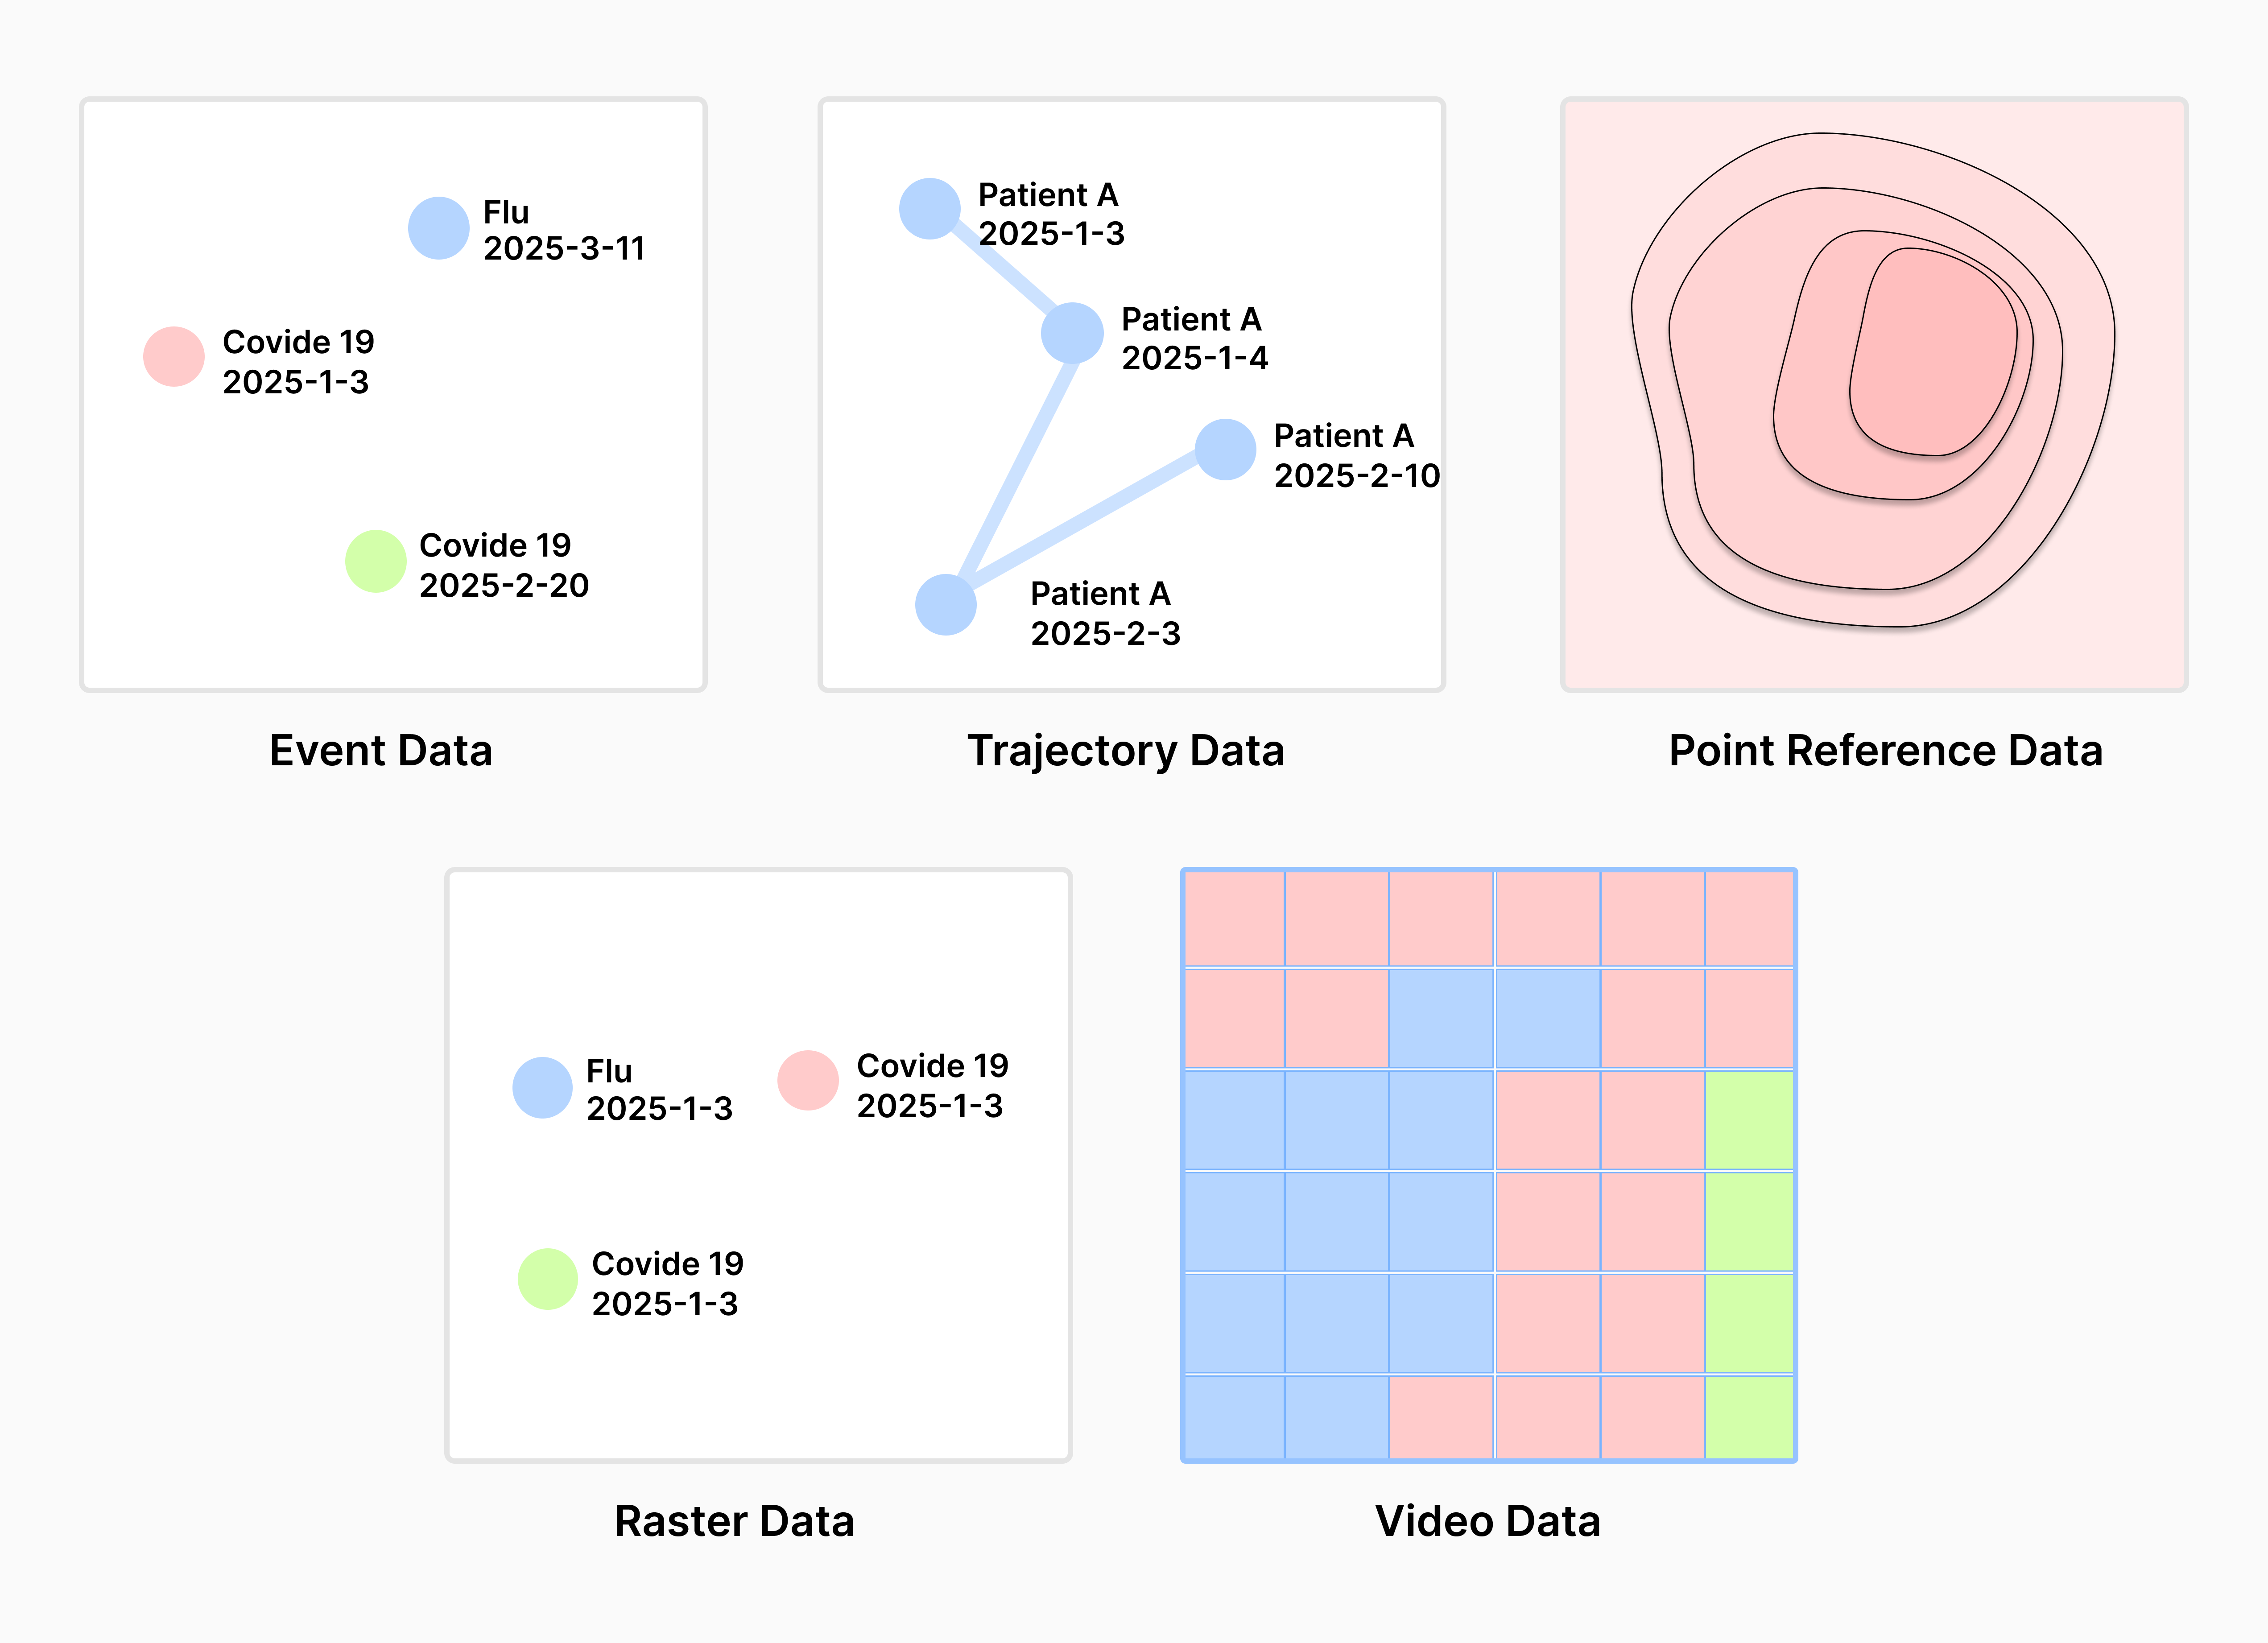
\includegraphics[width=0.6\linewidth]{Fivecategories.png}
    \caption{The five categories of spatiotemporal data in digital health---event, trajectory, point reference, raster, and video data---each shown with a representative clinical example (e.g., outbreak reports, wearable mobility traces, vital sign fields, hospital monitoring grids, and surgical video).}
    \Description{An illustration of the five categories of spatiotemporal data in digital health: event data, trajectory data, point-reference data, raster data, and video data, each paired with a representative clinical example.}
    \label{fig:Five Spatio temporal Data Categories}
\end{figure*}

\textbf{Event data} are discrete records in time and space, structured as (location, time, event type)---for example, confirmed infectious cases or outbreak reports for influenza or COVID-19---supporting risk prediction, anomaly detection, and transmission analysis.

\textbf{Trajectory data} describe an entity's path as an ordered series of (location, time) observations, arising from wearables, ambulance routing, or mobile screening units, and support path prediction, travel time estimation, and epidemiological analysis of movement.

\textbf{Point reference data} take the form (location, time, measurement), sampling a target field such as air quality, heart rate, or blood pressure at fixed locations, and support field interpolation, anomaly detection, and multisensor fusion.

\textbf{Raster data} are observations on fixed locations at regular intervals, forming a space--time tensor; examples include daily departmental outpatient volumes, fixed air quality stations, and fMRI time series, supporting spatiotemporal prediction, anomaly detection, and segmentation.

\textbf{Video data} are sequential image frames at high spatial and temporal resolution, appearing in surgical, ultrasound, and endoscopic recordings, and support lesion tracking, detection, and action recognition.

Much health data also carries relational structure, where measurements are linked by node--edge relations (road networks, brain functional connectivity, hospital referral networks). This is not a sixth category but a relational layer over the types above---most often point reference and raster data---where sites or regions become nodes and spatial, topological, or functional links become edges. Such data are handled by spatiotemporal graph neural networks (STGNN), discussed in Sections~\ref{sec:history} and~\ref{sec:models}.

Our primary interest is how patient covariates---behavior, exposure, physiology---vary jointly across space and time, so trajectory data is the most central form discussed, though the principles generalize across categories.

Public datasets make trajectory centric data increasingly feasible. StudentLife uses smartphone sensing to link day to day behavioral patterns with stress, sleep, sociability, and mental health outcomes~\cite{wang2014studentlife}, while harmonized multi site nutrition and biomarker efforts such as the NIH funded iPAT project add time indexed measurements and site level metadata for dietary pattern analysis in chronic disease research~\cite{Fang2021iPAT}. These resources let covariate--outcome relationships be examined spatiotemporally rather than as static summaries.

Downstream tasks on trajectory data fall into recurring goals: spatiotemporal feature aggregation, which summarizes how covariates evolve across time and context; prediction, which forecasts the next location or activity, future covariate values, or clinical risk by modeling movement in space and time; and intervention oriented reasoning, which identifies when and where actions are most likely to reduce risk, for example by linking mobility and context to lifestyle factors such as diet. These mirror the forecasting, representation learning, and decision support emphases of trajectory mining and mobility modeling.

Three strategies are common for processing trajectory data. Sequential modeling orders observations chronologically and applies recurrent, sequence to sequence, or attention based models to capture temporal dependencies, as in mobility and trajectory forecasting. Spatial mapping discretizes trajectories into grids or maps them onto structured supports such as road networks, after which convolutional modules emphasize local proximity. Hybrid modeling couples graph neural networks with temporal encoders over nodes and edges from road or interaction graphs, enforcing topological constraints and improving robustness under sparse sampling. These are elaborated in Sections~\ref{sec:history}--\ref{sec:models} and~\ref{sec:categorization} as CNN based, RNN based, Transformer based, and STGNN architectures.

\subsection{Challenges of Sparsity, Irregularity, and Multi-scale Structure in Spatiotemporal Health Data}
Although spatiotemporal models are well suited to digital health in principle, data challenges complicate deployment. Models benefit from dense, continuous observations, but health data are almost always sparse and irregularly sampled, constraining design, training, and evaluation.

Temporal sparsity is intrinsic: clinical follow up spans months or years yet observations are intermittent, with missingness from non-compliance, privacy, or operational limits. It is a defining property of longitudinal records and mobile sensing rather than an exception~\cite{che2018grud}.

Temporal irregularity compounds this: differing follow up schedules across sites yield highly uneven intervals that violate standard temporal model assumptions unless time gaps are modeled explicitly~\cite{shukla2021irregular}.

Spatial data span multiple granularities. Coarse location (residential or census level) is widely available in cohort datasets but sparse in spatial transitions, often missing contextual exposures. Fine grained mobility from wearables and mobile devices enables exposure estimation and context aware analysis but is noisy, incomplete, and unevenly available. The two scales are coupled---short term mobility is embedded in long term residence---so cross scale modeling must handle redundancy, confounding, and scale mismatch, with analogous short versus long term structure in the temporal dimension.

Together, sparsity, irregular sampling, heterogeneous spatial granularity, and cross scale dependency are the central challenges, requiring models robust to missing and irregular data that integrate information across spatial and temporal scales.

\section{History of Deep Learning--Based Spatiotemporal Modeling Methods in Digital Health}
\label{sec:history}
Having established the applicability of spatiotemporal data in digital health and its processing methods, this section reviews the historical development of spatiotemporal models across forecasting categories, then introduces the mainstream spatiotemporal models before turning to their digital health applications.

\subsection{The Historical Development of Spatiotemporal Models in Digital Health}
Historically, the exploration of deep learning for ST tasks commenced with simpler feed-forward networks such as Multilayer Perceptrons (MLPs). Early applications (pre-2015) adapted MLPs primarily for time-series prediction (e.g., forecasting disease incidence or patient visits~\cite{miotto2018deeplearning}), albeit with limited capacity to handle complex spatial relationships. Subsequently, RNNs and LSTMs gained prominence by extending the modeling scope to longer sequences and more nuanced temporal dynamics. By incorporating spatial structures into LSTM cells (e.g., ST-LSTM), these architectures could capture both spatial and temporal correlations, making them valuable in tasks like epidemic forecasting and wearable device data analytics.

Between 2015 and 2020, spatiotemporal graph neural networks (STGNN) and attention based mechanisms emerged. STGNNs added graph convolution to model non-Euclidean spatial relationships, from city wide traffic to hospital networks, while Transformers and variants such as ST-Transformer captured long range dependencies and enabled multimodal fusion of imaging, EHR, wearable, and environmental data~\cite{caroprese2018deepehr}.

Since 2020, spatiotemporal deep learning has combined Transformers, self-supervised learning, and multimodal fusion for fine grained dependencies, with exemplars such as TimeSformer and ST-Transformer variants for medical imaging sequences and climate health interactions~\cite{liu2024temporallearning}. Federated learning has concurrently emerged as a privacy preserving way to train across distributed medical datasets.

In parallel, statistics research has strengthened foundations useful for digital health spatiotemporal modeling: physics informed convection--diffusion models, Lagrangian cross-covariance functions, score driven models, semiparametric autoregressive models for irregular nonstationary locations, dynamic deformation covariance models, graphical models for nonstationary series, varying-coefficient disease mapping, spatial SIR emulators, and statistical deep learning syntheses~\cite{liu2022convectionDiffusion,salvana2023lagrangian,gasperoni2023scoreDriven,lu2024dyfast,castroMorales2025dynamicDeformation,basu2023graphicalNonstationary,wang2024respiratoryDiseaseMapping,trostle2024spatialSIR,wikle2023statisticalDeepLearning}. These contribute interpretable covariance structures, physical constraints, uncertainty quantification, and principled baselines for neural models.

We next introduce the foundational architectures (CNN, GNN, RNN, Transformer) and then the mainstream spatiotemporal model families: \emph{CNN--RNN hybrids}, which extract spatial features with CNNs and temporal dependencies with RNNs; \emph{spatiotemporal graph neural networks (STGNN)}, which model spatial relations on graphs with temporal encoders; \emph{Transformer based models}, which use self-attention for long range dependencies; and \emph{3D-CNN and hybrid networks} for high dimensional data such as video.

\begin{figure*}
    \centering
    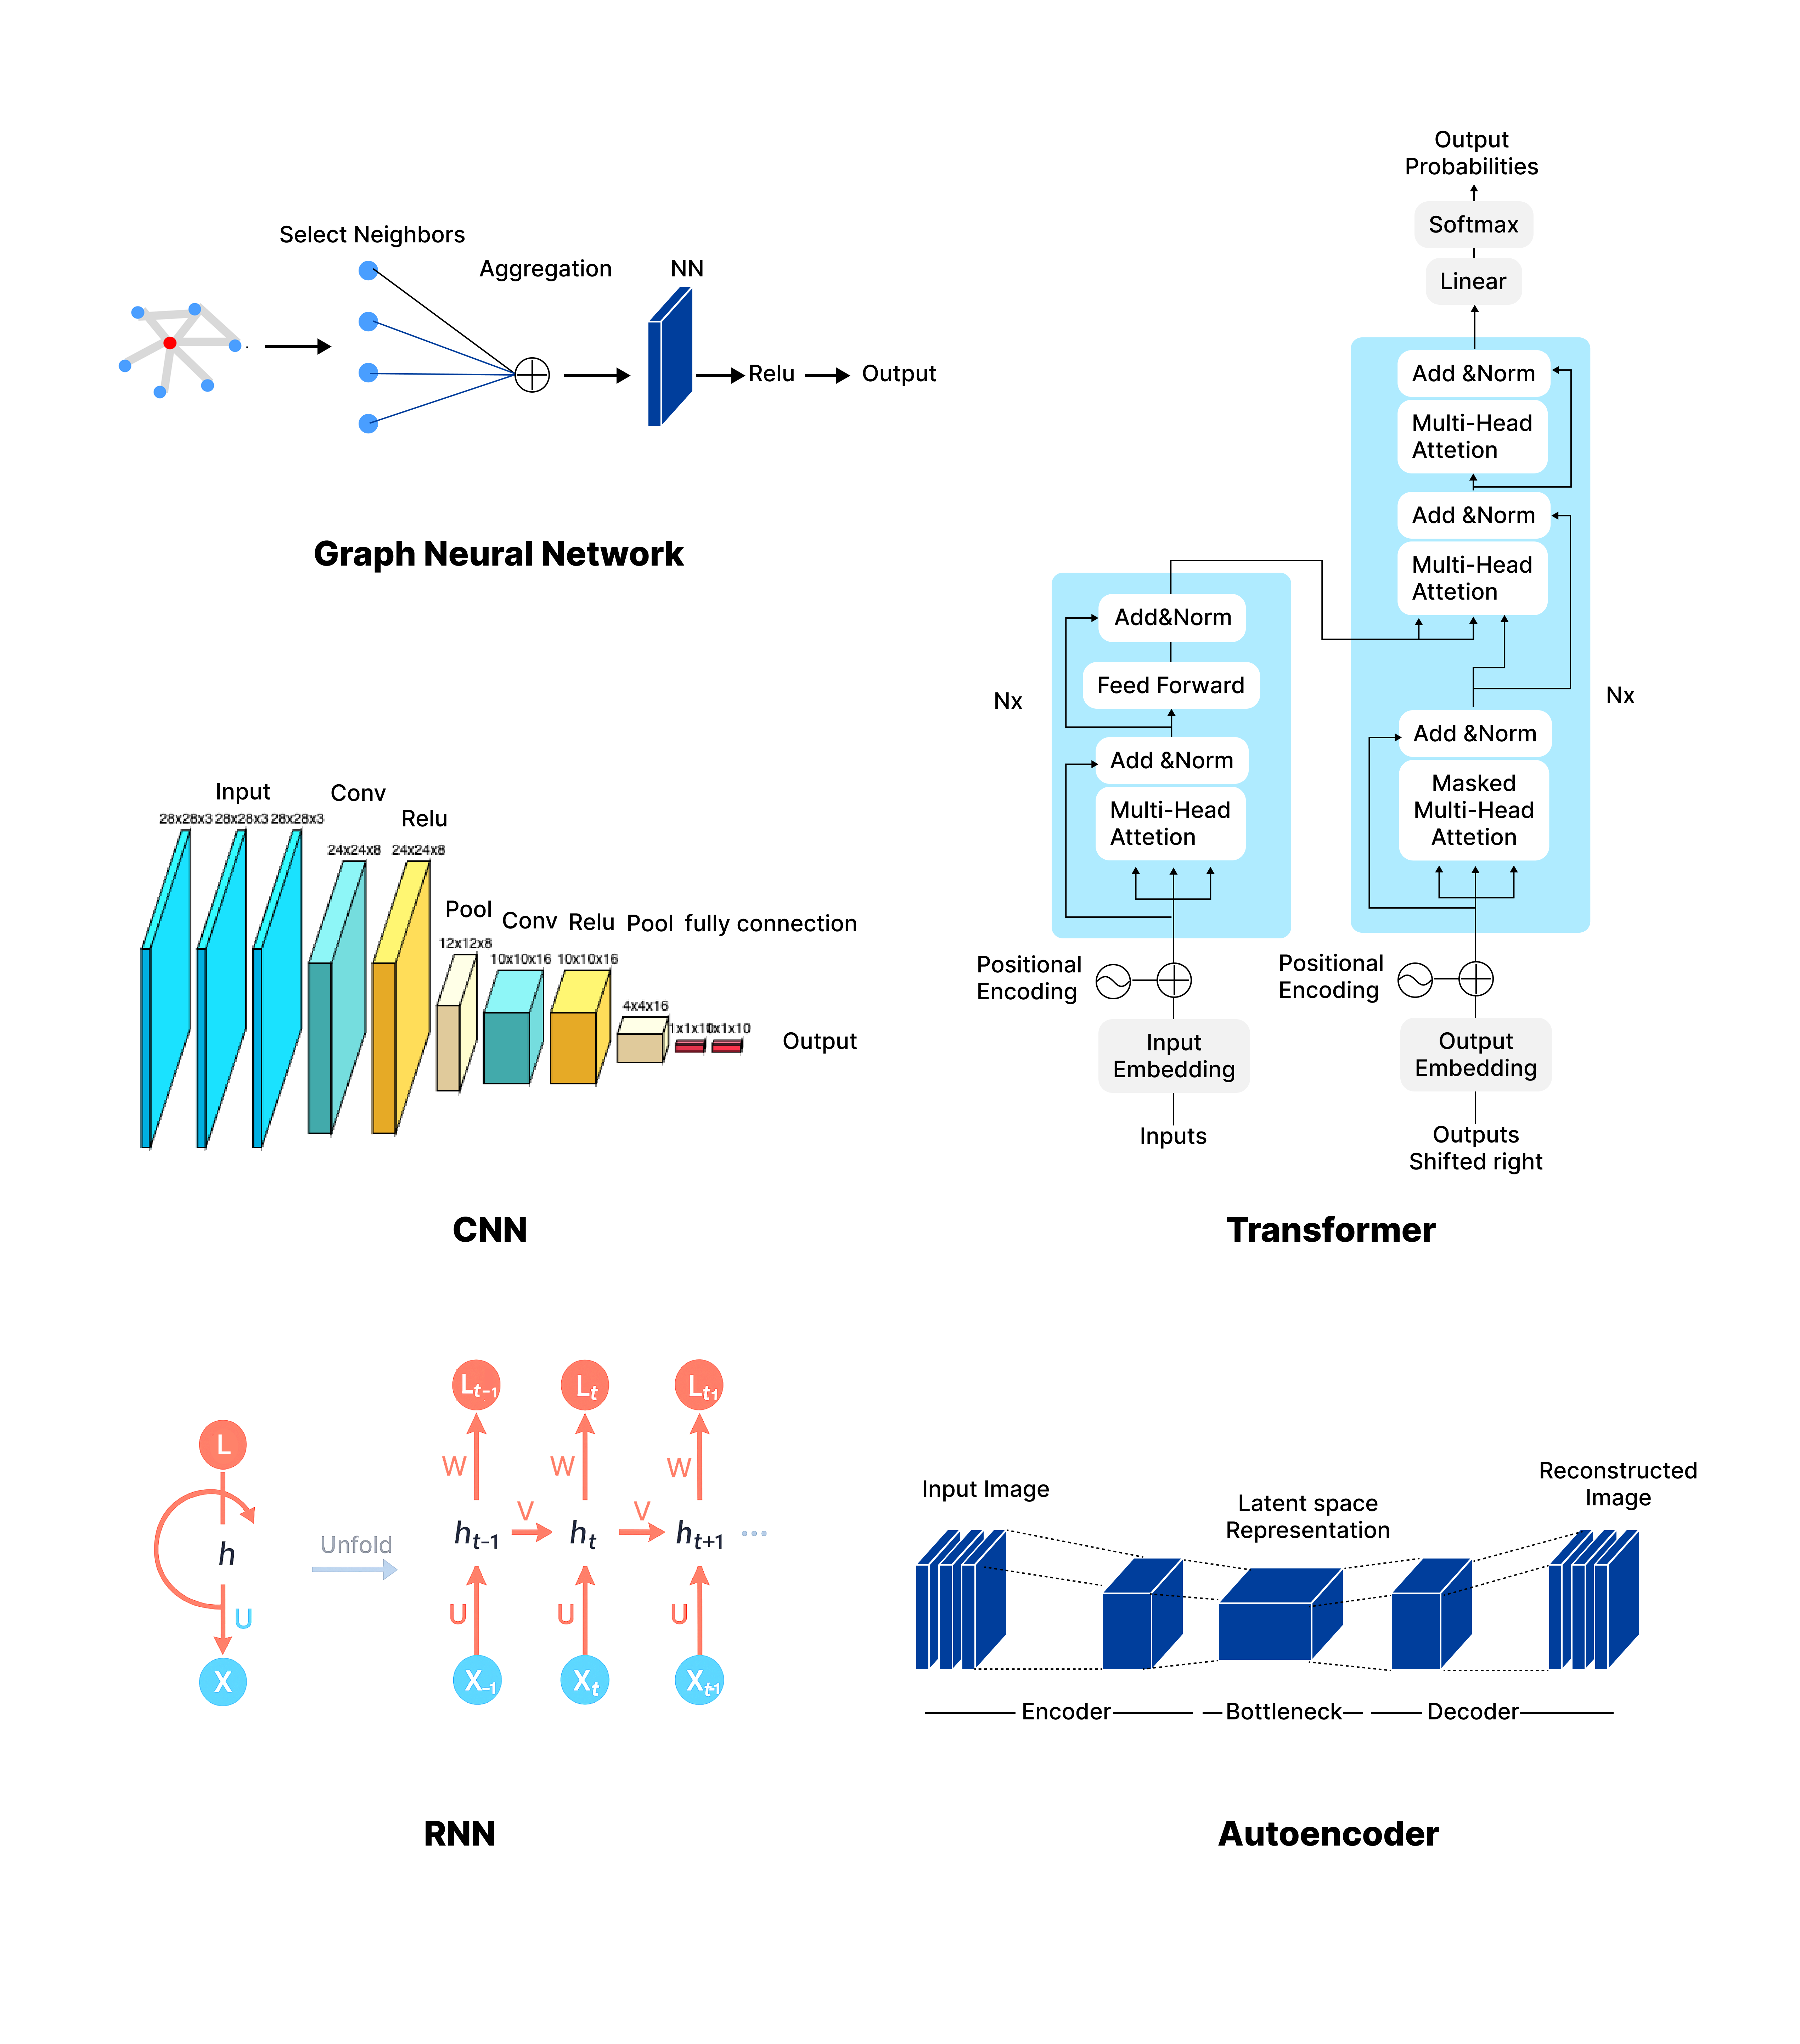
\includegraphics[width=\linewidth]{Frame 34.png}
    \caption{A general spatiotemporal modeling pipeline for digital health: foundational deep learning architectures (CNN, GNN, RNN, Transformer, and autoencoders) transform raw spatiotemporal health data into clinical predictions, forming the basis for the specialized model families surveyed in Sections~\ref{sec:history}--\ref{sec:categorization}. Figure~\ref{fig:foundation_arch} details the internal structure of several of these architectures.}
    \Description{A schematic of a general spatiotemporal modeling pipeline for digital health, showing how raw spatiotemporal health data are encoded by foundational deep learning architectures (CNN, GNN, RNN, Transformer, and autoencoders) and mapped to clinical prediction tasks.}
    \label{fig:GeneralModel}
\end{figure*}

\subsection{Foundational Deep Learning Architectures }
These architectures underpin many spatiotemporal models. We briefly review GNNs~\cite{scarselli2009gnn}, RNNs~\cite{rumelhart1986rnn}, Transformers~\cite{vaswani2017attention}, autoencoders~\cite{hinton2006reducing} and stacked variants~\cite{masci2011stacked}, state space models including Mamba~\cite{gu2023mamba}, GANs~\cite{goodfellow2014gan}, denoising diffusion models (DDPMs)~\cite{ho2020ddpm}, and world models~\cite{maes2026leworldmodel} (Figures~\ref{fig:GeneralModel} and~\ref{fig:foundation_arch}) before turning to specialized techniques.


\paragraph{Graph Neural Networks (GNNs)}: Many systems---social, molecular, transportation, recommendation---are graph structured, where grid and sequence models such as CNNs~\cite{lecun1998cnn} and RNNs struggle. GNNs~\cite{scarselli2009gnn} process a graph $G=(V,E)$ with node features by message passing: each node aggregates information from its neighbors and updates its embedding. At layer $l$,
\begin{equation}
m_i^{(l)} = \sum_{j \in N(i)} f\bigl(h_j^{(l-1)}, h_i^{(l-1)}, e_{ij}\bigr), \quad h_i^{(l)} = \sigma\bigl(W m_i^{(l)} + b\bigr),
\end{equation}
where $f(\cdot)$ is the aggregation function, $e_{ij}$ an optional edge feature, and $W,b,\sigma$ the trainable transform and activation. Variants differ in aggregation: GCN uses spectral convolution~\cite{kipf2017gcn}, GAT attention weighted neighbors~\cite{velickovic2018gat}, and GIN MLP based updates for greater expressiveness~\cite{xu2019gin}.

\paragraph{Recurrent Neural Networks (RNN) and Variants}: RNNs~\cite{rumelhart1986rnn} model sequences through a hidden state $h_t = f(W_h h_{t-1} + W_x x_t + b_h)$ that carries past context, but suffer from vanishing and exploding gradients on long sequences. Long Short-Term Memory (LSTM)~\cite{rnn_lstm} adds input, forget, and output gates and a cell state that together retain long term information while discarding irrelevant detail; Gated Recurrent Units simplify this with fewer gates.

\paragraph{Transformer}: The Transformer~\cite{vaswani2017attention} stacks encoder and decoder layers of multi-head self-attention, feedforward networks, residual connections, and layer normalization, with causal masking in the decoder. Self-attention projects the input $X$ into queries, keys, and values $Q,K,V$ and computes
\begin{equation}
\mathrm{Attention}(Q,K,V) = \mathrm{softmax}\!\left(\frac{QK^\top}{\sqrt{d_k}}\right) V,
\end{equation}
where $d_k$ scales the scores. Computing all pairwise interactions in parallel lets Transformers capture long range dependencies efficiently.

\paragraph{AutoEncoder (AE) and Stacked AutoEncoder (SAE)}: An autoencoder learns an encoder that maps input $\mathbf{x}$ to a latent code $\mathbf{h}$ and a decoder that reconstructs $\hat{\mathbf{x}}$, trained to minimize reconstruction error; Hinton and Salakhutdinov~\cite{hinton2006reducing} introduced deep AEs for dimensionality reduction. In spatiotemporal modeling, AEs extract local spatial and temporal patterns for tasks such as traffic and environmental monitoring~\cite{vincent2008extracting, bengio2009learning}. Stacked AEs deepen this through layerwise pretraining and fine tuning for multiscale features~\cite{erhan2010why, ranzato2007unsupervised, masci2011stacked, vincent2010stacked}, while Variational AEs~\cite{kingma2013auto} add a probabilistic latent space for representation and generation~\cite{glorot2010understanding, zhang2017deep, yu2018spatio}.

\paragraph{State-Space Models and Mamba}: State-space models (SSMs) propagate a latent state linearly over time, an efficient alternative to attention for long sequences. After discretization,
\begin{equation}
h_t = \bar{A} h_{t-1} + \bar{B} x_t, \quad y_t = C h_t,
\end{equation}
which, being linear, can be unrolled as a global convolution for efficient long sequence training, as in the S4 family~\cite{smith2023convssm}. Mamba~\cite{gu2023mamba} makes the parameters input dependent (selective), keeping linear time, constant memory inference. These properties suit long physiological streams (continuous glucose, ECG, EEG), long video, and multi-year trajectories where self-attention is too costly.

\paragraph{Generative Adversarial Networks (GANs)}: GANs~\cite{goodfellow2014gan} pit a generator $G$ that maps noise $z$ to samples against a discriminator $D$ that separates real from synthetic, trained on the minimax objective
\begin{equation}
\min_G \max_D \; \mathbb{E}_{x \sim p_{\text{data}}}[\log D(x)] + \mathbb{E}_{z \sim p_z}[\log (1 - D(G(z)))].
\end{equation}
At convergence $G$ matches the data distribution. In digital health, GANs synthesize medical images and physiological signals, augment scarce or imbalanced cohorts, and impute missing values; conditional and temporal variants generate context conditioned spatiotemporal sequences.

\paragraph{Denoising Diffusion Probabilistic Models (DDPMs)}: DDPMs~\cite{ho2020ddpm} corrupt data with Gaussian noise over $T$ steps according to a schedule $\{\beta_t\}$,
\begin{equation}
q(x_t \mid x_{t-1}) = \mathcal{N}\!\left(x_t; \sqrt{1-\beta_t}\, x_{t-1}, \; \beta_t \mathbf{I}\right),
\end{equation}
and train a network $\epsilon_\theta$ to reverse it by predicting the added noise, $L = \mathbb{E}_{x_0,\epsilon,t}[\|\epsilon - \epsilon_\theta(x_t,t)\|^2]$. Sampling iteratively denoises from pure noise. Compared with GANs, diffusion offers more stable training and higher fidelity, and is increasingly used for high fidelity generation and denoising of medical images and signals, imputation of irregular measurements, and augmentation for downstream prediction.

\paragraph{World Models}: World models learn a compact model of how an environment evolves so that future states can be predicted and actions evaluated by simulation~\cite{ha2018worldmodels}. Joint-Embedding Predictive Architectures (JEPA) encode observations into a latent state and predict its evolution~\cite{lecun2022jepa,maes2026leworldmodel}: an encoder $E_\theta$ maps $x_t$ to $z_t$, a predictor $P_\phi$ rolls it forward under action $a_t$, and training aligns the prediction with a target encoded future,
\begin{equation}
\begin{aligned}
z_t &= E_\theta(x_t), \quad \hat{z}_{t+1} = P_\phi(z_t, a_t),\\
L &= \left\| \hat{z}_{t+1} - E_{\bar{\theta}}(x_{t+1}) \right\|^2,
\end{aligned}
\end{equation}
with $E_{\bar{\theta}}$ a slowly updated target encoder. In digital health, world models support patient state simulation and counterfactual planning and underpin the world model based digital twins of Section~\ref{sec:world_model_dt}.

\begin{figure*}
    \centering
    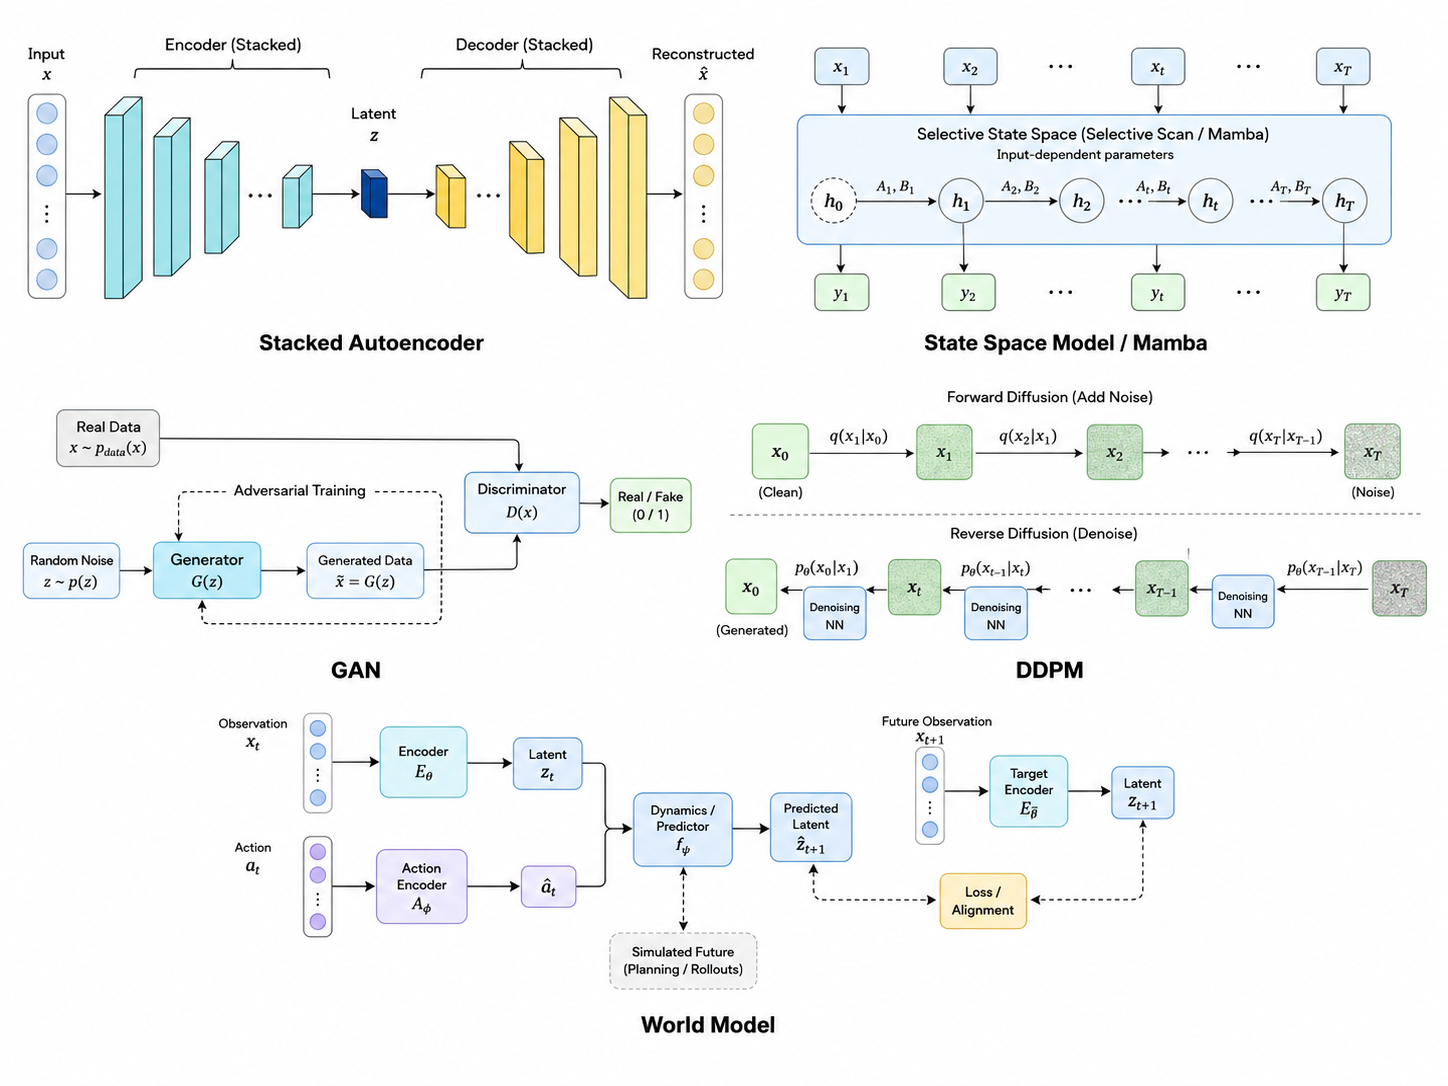
\includegraphics[width=\linewidth]{arch2.png}
    \caption{Internal structure of five foundational deep learning architectures, complementing the pipeline overview in Figure~\ref{fig:GeneralModel}. The stacked autoencoder compresses an input into a latent code and reconstructs it through stacked encoder and decoder layers; the state space model (Mamba) propagates an input dependent hidden state across time through a selective scan; the generative adversarial network (GAN) trains a generator against a discriminator that separates real from synthetic samples; the denoising diffusion probabilistic model (DDPM) corrupts data with noise in a forward process and learns to reverse it to generate clean samples; and the world model encodes an observation and an action into a latent state, predicts the next latent state, and aligns it with a target encoding of the future observation to support simulation and planning.}
    \Description{Five panels showing the architectures of a stacked autoencoder, a state space model (Mamba), a generative adversarial network, a denoising diffusion probabilistic model, and a world model, each drawn as a block diagram with its inputs, latent states, and outputs.}
    \label{fig:foundation_arch}
\end{figure*}


% \subsection{Spatiotemporal Model}
% While general DNN frameworks like Transformers and AEs excel at feature learning, many real world challenges involve both space and time dimensions. In this section, we shift our focus to Spatiotemporal models, which integrate spatial feature extraction with temporal sequence modeling. These models address tasks such as traffic prediction, meteorological forecasting, and video analysis by capturing interactions across both space and time. We will explore various architectures—from 3D CNN, CNN-RNN hybrids to graph-based and Transformer-based solutions that build upon the fundamentals described in the previous section.

% \paragraph{CNN-RNN Hybrid Model}The CNN-RNN hybrid model is one of the earliest deep learning architectures applied to ST modeling. This model extracts spatial features using Convolutional Neural Networks (CNN) and learns temporal dependencies using Recurrent Neural Networks (RNN), such as Long Short-Term Memory (LSTM) or Gated Recurrent Units (GRU). This approach has demonstrated effectiveness in tasks like weather forecasting and video analysis. For instance, Li et al.~\cite{li2025solar} proposed a hybrid deep learning framework for solar radiation forecasting, utilizing CNN for spatial feature extraction and LSTM for capturing temporal dependencies, significantly improving prediction accuracy. However, a major drawback of this model is its high computational complexity and the potential vanishing gradient problem when dealing with long-term dependencies.

% \paragraph{ST Graph Neural Networks (STGNN)} ST Graph Neural Networks (STGNN) \cite{shao2022longterm} have gained significant attention for modeling complex, non-Euclidean spatial data, such as traffic flow and power grid monitoring. STGNNs utilize Graph Neural Networks (GNN) to model spatial relationships between nodes while employing temporal models like LSTM or Transformer to learn temporal evolution patterns. For example, Wang et al.~\cite{wang2025rul} proposed a Graph Feature Attention Network (GFAN)-based method for predicting the remaining useful life of multi-sensor systems, effectively capturing ST dependencies between sensors. Although STGNNs perform well in many applications, they are computationally expensive and require significant resources for large-scale graph data processing.

% \paragraph{Transformer-based ST model} Transformer-based ST models have become a research hotspot in recent years. The self-attention mechanism in Transformer architectures allows them to capture long-range dependencies effectively, making them highly suitable for ST sequence modeling. Unlike traditional RNN-based models, Transformers handle long-term dependencies more efficiently. For example, Yu et al.~\cite{yu2025graph} introduced a method integrating dynamic Transformers with Graph Diffusion Learning (GDL) to improve anomaly detection in multivariate time series. Additionally, Wang et al.~\cite{wang2025propeller} developed a Transformer-SMFANet-based model to enhance the accuracy of propeller wake predictions. While Transformer-based models have made significant breakthroughs in ST forecasting, their high computational cost and dependence on large-scale data remain major challenges.

\paragraph{Patient State Simulation and Planning}: Counterfactual patient state simulation extends spatiotemporal learning from prediction toward intervention planning. Because it depends on both latent dynamics and synchronized digital twin infrastructure, we discuss it with world model based digital twins in Section~\ref{sec:world_model_dt}.

\paragraph{CNN-RNN Hybrid Model}
The CNN--RNN hybrid is one of the earliest spatiotemporal architectures and remains widely used: a CNN extracts spatial features from grid structured inputs, and a recurrent module models their temporal evolution.
 
At each step, a spatial snapshot $X_t \in \mathbb{R}^{H \times W \times C}$ (image, sensor heatmap, or gridded field) is encoded by the CNN into a feature vector $z_t$; the sequence $\{z_1,\ldots,z_T\}$ is then fed to a recurrent network, typically an LSTM~\cite{rnn_lstm} or GRU~\cite{cho2014gru}, which models its temporal evolution.
 
ConvLSTM~\cite{shi2015convolutional} replaces the dense operations in LSTM gates with convolutions, preserving spatial structure and proving effective for precipitation nowcasting. Hybrids have since served solar forecasting~\cite{li2025solar}, video prediction~\cite{srivastava2015unsupervised}, action recognition~\cite{donahue2015longterm}, and medical imaging time series, where the spatial branch captures anatomy and the temporal branch tracks disease progression.
 
Their limitations are well known: CNNs assume regular grids and cannot handle irregular structures such as road or referral networks (motivating graph models); RNNs process steps sequentially, limiting parallelism and long range dependency learning~\cite{bengio1994learning}; and the two-stage design separates spatial and temporal modeling, which more tightly coupled models such as ConvLSTM and attention based architectures improve on.
 
\paragraph{Spatiotemporal Graph Neural Networks (STGNN)}
Spatiotemporal graph neural networks (STGNN)~\cite{shao2022longterm} model non-Euclidean spatial relationships with temporal dynamics. Rather than grids, they represent space as a graph $G=(V,E)$ whose nodes are entities (sensors, hospitals, brain regions) and edges encode proximity, functional connectivity, or administrative links, capturing irregular topologies common in real systems.
 
STGNNs alternate spatial aggregation and temporal layers. In the spatial layer, each node aggregates neighbor features via a GCN~\cite{kipf2017gcn}, GAT~\cite{velickovic2018gat}, or message passing operator; for node $i$ at layer $l$:
 
\begin{equation}
h_i^{(l)} = \sigma \Bigl( \sum_{j \in \mathcal{N}(i)} \alpha_{ij} \, W^{(l)} h_j^{(l-1)} + b^{(l)} \Bigr)
\end{equation}
 
where $\alpha_{ij}$ is the edge weight or attention coefficient and $W^{(l)},b^{(l)},\sigma$ are the learnable transform and activation. Temporal layers then process the per step representations with LSTM~\cite{rnn_lstm}, GRU~\cite{cho2014gru}, temporal convolution~\cite{lea2017temporal}, or attention~\cite{vaswani2017attention}.
 
Landmark designs include DCRNN~\cite{li2018dcrnn} (diffusion convolution with an encoder--decoder GRU), STGCN~\cite{yu2018spatio} (graph plus 1D temporal convolutions, avoiding recurrence), Graph WaveNet~\cite{wu2019graphwavenet} (an adaptive adjacency matrix with dilated causal convolutions), ASTGCN~\cite{guo2019astgcn} (spatial and temporal attention for nonstationary data), and a GFAN based method~\cite{wang2025rul} for remaining useful life of multi-sensor systems.
 
STGNNs perform strongly on traffic~\cite{yu2018spatio, li2018dcrnn}, air quality, power grid, and brain connectivity tasks, but face challenges: graph construction needs domain knowledge and can bias results; large node counts make adjacency operations costly, partly mitigated by sampling~\cite{hamilton2017inductive}, sparsification, and mini-batch training; and most assume a static topology, so dynamic graphs remain an open problem~\cite{pareja2020evolvegcn}.
 
\paragraph{Transformer-Based Spatiotemporal Models}
Transformer based spatiotemporal models offer an alternative to recurrent and graph-convolutional architectures: self-attention~\cite{vaswani2017attention} computes all pairwise interactions in parallel, avoiding the recurrent bottleneck and capturing long range dependencies.
 
Adapting them to spatiotemporal data means attending across spatial tokens (locations or nodes) and across time, with positional encodings from coordinates and timestamps to restore ordering that permutation invariant attention would otherwise discard.
 
STTNet~\cite{xu2020stransformer} factorizes spatial and temporal attention, cutting complexity from $O((N \times T)^2)$ to $O(N^2 + T^2)$ for $N$ locations and $T$ steps; Traffic Transformer~\cite{cai2020traffic} restricts attention to spatially proximate nodes via a graph mask; and TimeSformer~\cite{bertasius2021timesformer} uses divided space-time attention for efficient action recognition.
 
Recent variants push efficiency and structure: dynamic Transformers with graph diffusion learning for anomaly detection~\cite{yu2025graph}, a Transformer-SMFANet for propeller wake prediction~\cite{wang2025propeller}, Informer~\cite{zhou2021informer} with ProbSparse attention at $O(T \log T)$, and Autoformer~\cite{wu2021autoformer} with series decomposition for long horizon forecasting.
 
Open challenges remain: the quadratic cost of attention is prohibitive for very large domains or horizons; pretraining on spatiotemporal corpora is limited by data availability; and the lack of locality and graph inductive biases can cause underfitting in low data regimes, motivating hybrids with convolution or graph structure.
 
% \begin{figure*}
%     \centering
%     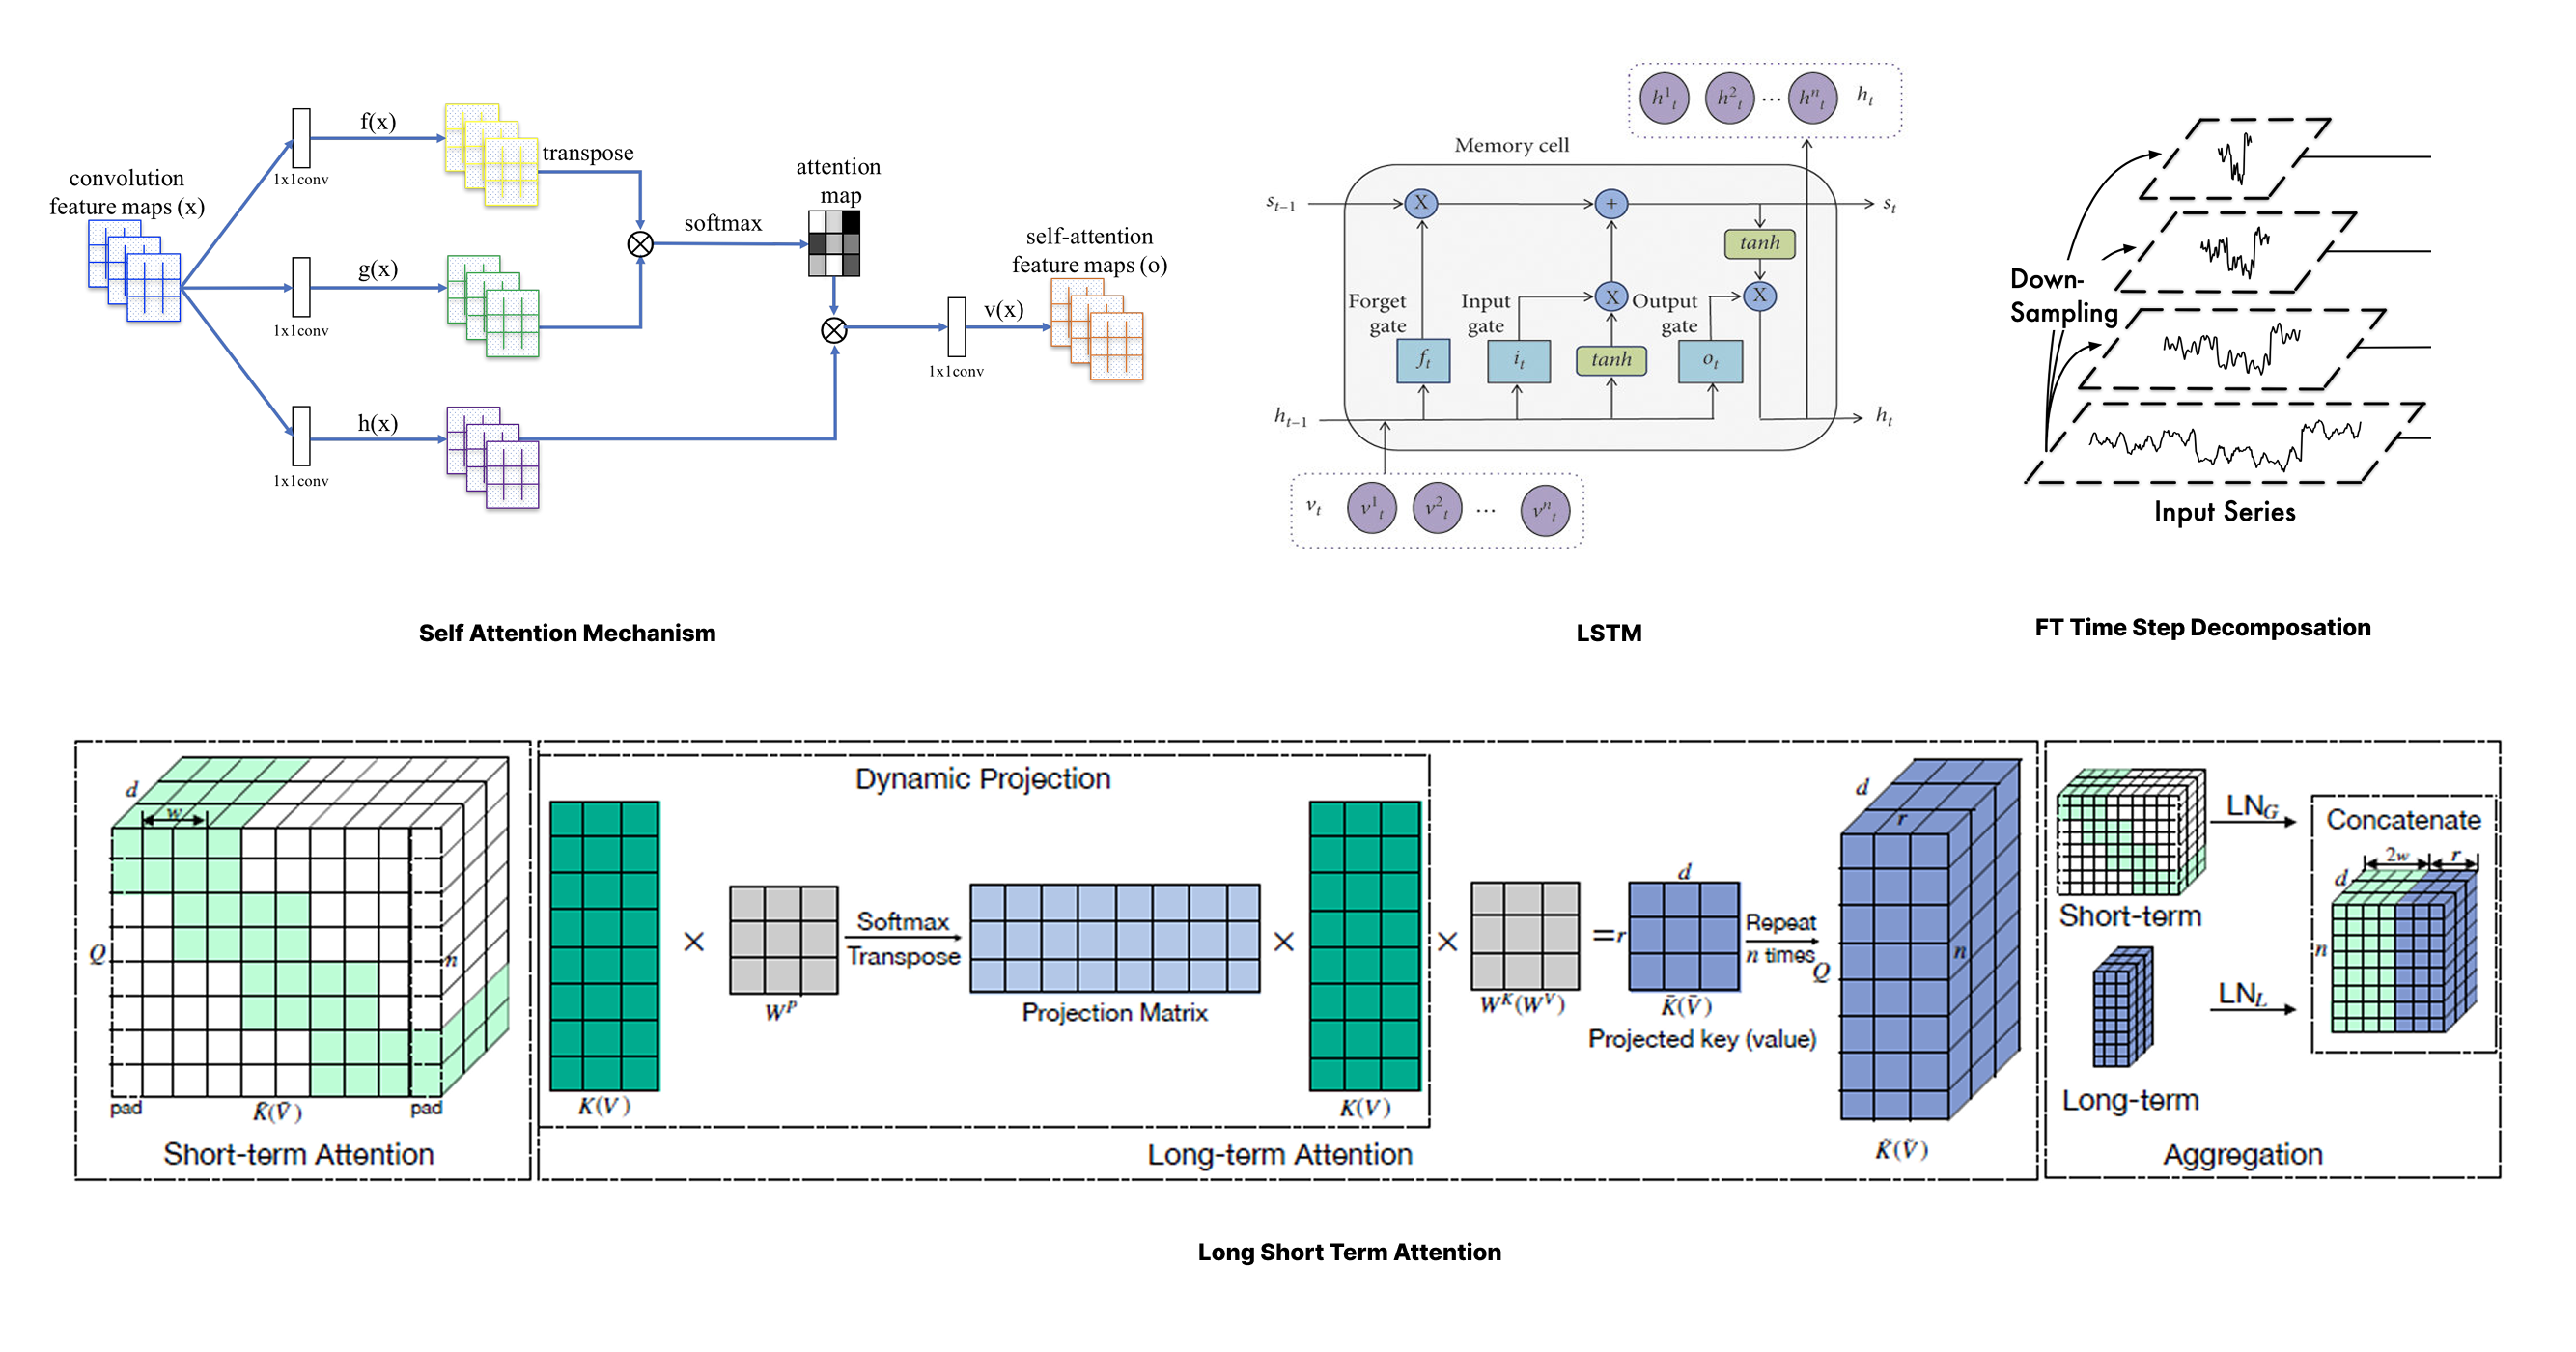
\includegraphics[width=1\linewidth]{temporal (1).png}
%     \caption{Temporal Model}
%     \label{Temporal Model}
%     \Description{Temporal Model}
% \end{figure*}
\begin{table*}[htbp]
\centering
\caption{Comparison of Deep Learning--Based Spatiotemporal Architectures for Digital Health Applications}
\label{tab:st-model-comparison}
\footnotesize
\renewcommand{\arraystretch}{1.0}
\begin{tabularx}{\textwidth}{>{\raggedright\arraybackslash}p{2.2cm} >{\raggedright\arraybackslash}p{2.5cm} >{\raggedright\arraybackslash}p{2.5cm} >{\raggedright\arraybackslash}p{1.4cm} >{\raggedright\arraybackslash}p{1.8cm} >{\raggedright\arraybackslash}X}
\toprule
\textbf{Model Type} & \textbf{Spatial Handling} & \textbf{Temporal Handling} & \textbf{Comp. Cost} & \textbf{Data Needs} & \textbf{Digital Health Examples} \\
\midrule
 
CNN-RNN Hybrid
& CNN extracts local spatial features via convolutional filters on grid-structured inputs (e.g., images, spatial maps)
& RNN/LSTM/GRU models sequential dependencies through recurrent hidden states
& Moderate to High
& Moderate; requires spatially gridded or image-like data with temporal ordering
& Medical image sequence analysis; wearable sensor forecasting; regional disease incidence prediction \\
 
\addlinespace[4pt]
 
STGNN
& GNN (GCN, GAT) propagates information over graph-structured spatial relationships (non-Euclidean)
& Temporal modules (LSTM, GRU, or temporal convolution) capture evolution along the time axis
& High
& Requires explicit graph structure (e.g., adjacency matrix); moderate to large labeled data
& Hospital network patient flow; multi-sensor physiological monitoring; epidemic spread over contact/mobility networks \\
 
\addlinespace[4pt]
 
Transformer-based ST
& Self-attention over spatial tokens or positional embeddings; no fixed spatial inductive bias
& Self-attention with temporal positional encoding captures long-range dependencies in parallel
& High to Very High
& Large-scale data preferred; benefits from pre-training; positional encoding needed for spatial structure
& Large-scale EHR longitudinal prediction; climate--health interaction modeling; multi-modal medical data fusion \\

\addlinespace[4pt]

3D-CNN \& Hybrid Networks
& 3D convolution jointly captures spatial patterns across height, width, and depth/time dimensions
& Temporal dynamics learned implicitly through the depth axis of 3D convolution kernels
& High
& High-dimensional volumetric or video-like data (e.g., $H \times W \times T$)
& Medical video analysis (e.g., echocardiography, surgical video); fMRI/brain imaging sequences; motion-based rehabilitation assessment \\

\addlinespace[4pt]

AE / SAE / VAE
& Encoder compresses spatial features into a latent space; can be combined with CNN or GNN encoders
& Temporal patterns captured when paired with sequential encoders or applied per time step
& Low to Moderate
& Can leverage unlabeled data (unsupervised / self-supervised); flexible input formats
& Anomaly detection in patient vitals; missing data imputation in longitudinal records; latent phenotype discovery from EHR \\

\addlinespace[4pt]

State-Space Models / Mamba
& Spatial structure handled implicitly through tokenization or combined with CNN/GNN encoders; no built-in spatial bias
& Selective state-space recurrence captures long-range temporal dependencies in linear time
& Low to Moderate
& Efficient on very long sequences; moderate labeled data
& Long continuous physiological streams (CGM, ECG, EEG); long-horizon longitudinal trajectories; long medical video \\

\addlinespace[4pt]

GAN
& Generator and discriminator use CNN or GNN backbones to model spatial structure
& Temporal dynamics modeled by recurrent or temporal convolution generators (conditional or temporal GAN variants)
& Moderate to High
& Augments scarce or imbalanced cohorts; benefits from moderate real samples
& Synthetic medical image and signal generation; data augmentation for rare conditions; missing value imputation \\

\addlinespace[4pt]

DDPM (Diffusion)
& U-Net (CNN) backbone captures spatial structure during iterative denoising
& Temporal or spatiotemporal dynamics modeled by conditioning the denoiser on time or sequence context
& High
& Moderate to large data; stable training with high sample fidelity
& High-fidelity medical image and signal synthesis and denoising; imputation of irregular measurements; data augmentation \\

\addlinespace[4pt]

World Model
& Encoder (CNN, GNN, or Transformer) maps observations into a latent state representing spatial context
& Latent dynamics model rolls the state forward over time for prediction and simulation
& High
& Sequential observation and action data; benefits from large interaction data
& Patient-state simulation; counterfactual intervention planning; world model based digital twins \\

\bottomrule
\end{tabularx}

{\footnotesize \textit{Note:} Computational cost is characterized relative to other architectures in this table. Actual cost depends on data scale, graph size, sequence length, and implementation details.}
\end{table*}

 
 
\subsection{Irregular Time Series and Longitudinal Modeling in Digital Health}
We include irregular time series and longitudinal modeling because they form the temporal backbone of spatiotemporal learning under real-world digital health constraints: irregular sampling and personalized, nonstationary trajectories are exactly what spatial and contextual covariates must align with, extending rather than departing from the framework of Sections~\ref{sec:data}--\ref{sec:history}. Beyond the general models above, digital health adds nonstationarity, irregular sampling, and personalized trajectories, motivating the specialized methods below.

\paragraph{Hybrid long and short term models}: Hybrid designs feed LSTM encoded short term features into a Transformer, using self-attention for the long range dependencies that gated recurrence captures poorly, giving robust performance when both fluctuations and trends matter.

\paragraph{TimeMixer}: TimeMixer~\cite{timemixer} applies MLP token mixing over sliding windows and adds a Fourier decomposition $X_f=\mathrm{FFT}(X)$, where low and high frequency bands capture long term trends and short term variation, improving periodic pattern learning.

\paragraph{Trajectory representation learning}: Spatiotemporal hypergraph models for next point of interest recommendation~\cite{Zhang2023POI} represent an individual's history as a longitudinal trajectory of locations and timestamps, with hyperedges over users, places, and time contexts capturing higher order interactions beyond pairwise relations. Replacing points of interest with health contexts (environments, behaviors, exposures) and the target with disease risk reuses the same representation for personalized health prediction.

\paragraph{MICN}: MICN~\cite{wang2023micn} fuses multi-scale convolution---small kernels for short term fluctuations, large kernels for long term trends---with a Transformer over time steps, suiting air quality, weather, and traffic forecasting.

\paragraph{Periodic and frequency based models}: Periodic Transformers add periodic encoding for cyclical variation under irregular sampling, and FEDformer combines frequency and time domain modeling for strongly periodic sequences~\cite{zhou2022fedformer}; wavelet transforms further aid joint temporal and spectral feature extraction.

\paragraph{Time aware models for irregular sampling}: Standard RNNs assume uniform intervals. GRU-$\Delta t$~\cite{metzger2023crop} adds a decay $\Gamma(\Delta t)=e^{-\Delta t/\tau}$ so older information fades as the gap $\Delta t$ grows, handling irregular medical and sensor streams.

ODE-RNN~\cite{rubanova2019latent} couples Neural ODEs~\cite{chen2018neural} with RNNs, evolving the hidden state continuously via $\frac{dh}{dt}=f(h,t;\theta)$ between observations and updating it discretely on arrival, capturing both smooth trends and sudden changes for ECG/EEG and epidemiological data.

Transformer variants extend this idea: ContiFormer~\cite{chen2023contiformer} embeds Neural ODEs in attention for continuous time, and Rough Transformers~\cite{morenopino2024rough} use rough path (signature) features for noisy, unevenly sampled ICU data.

% \begin{figure*}[t]
%     \centering
%     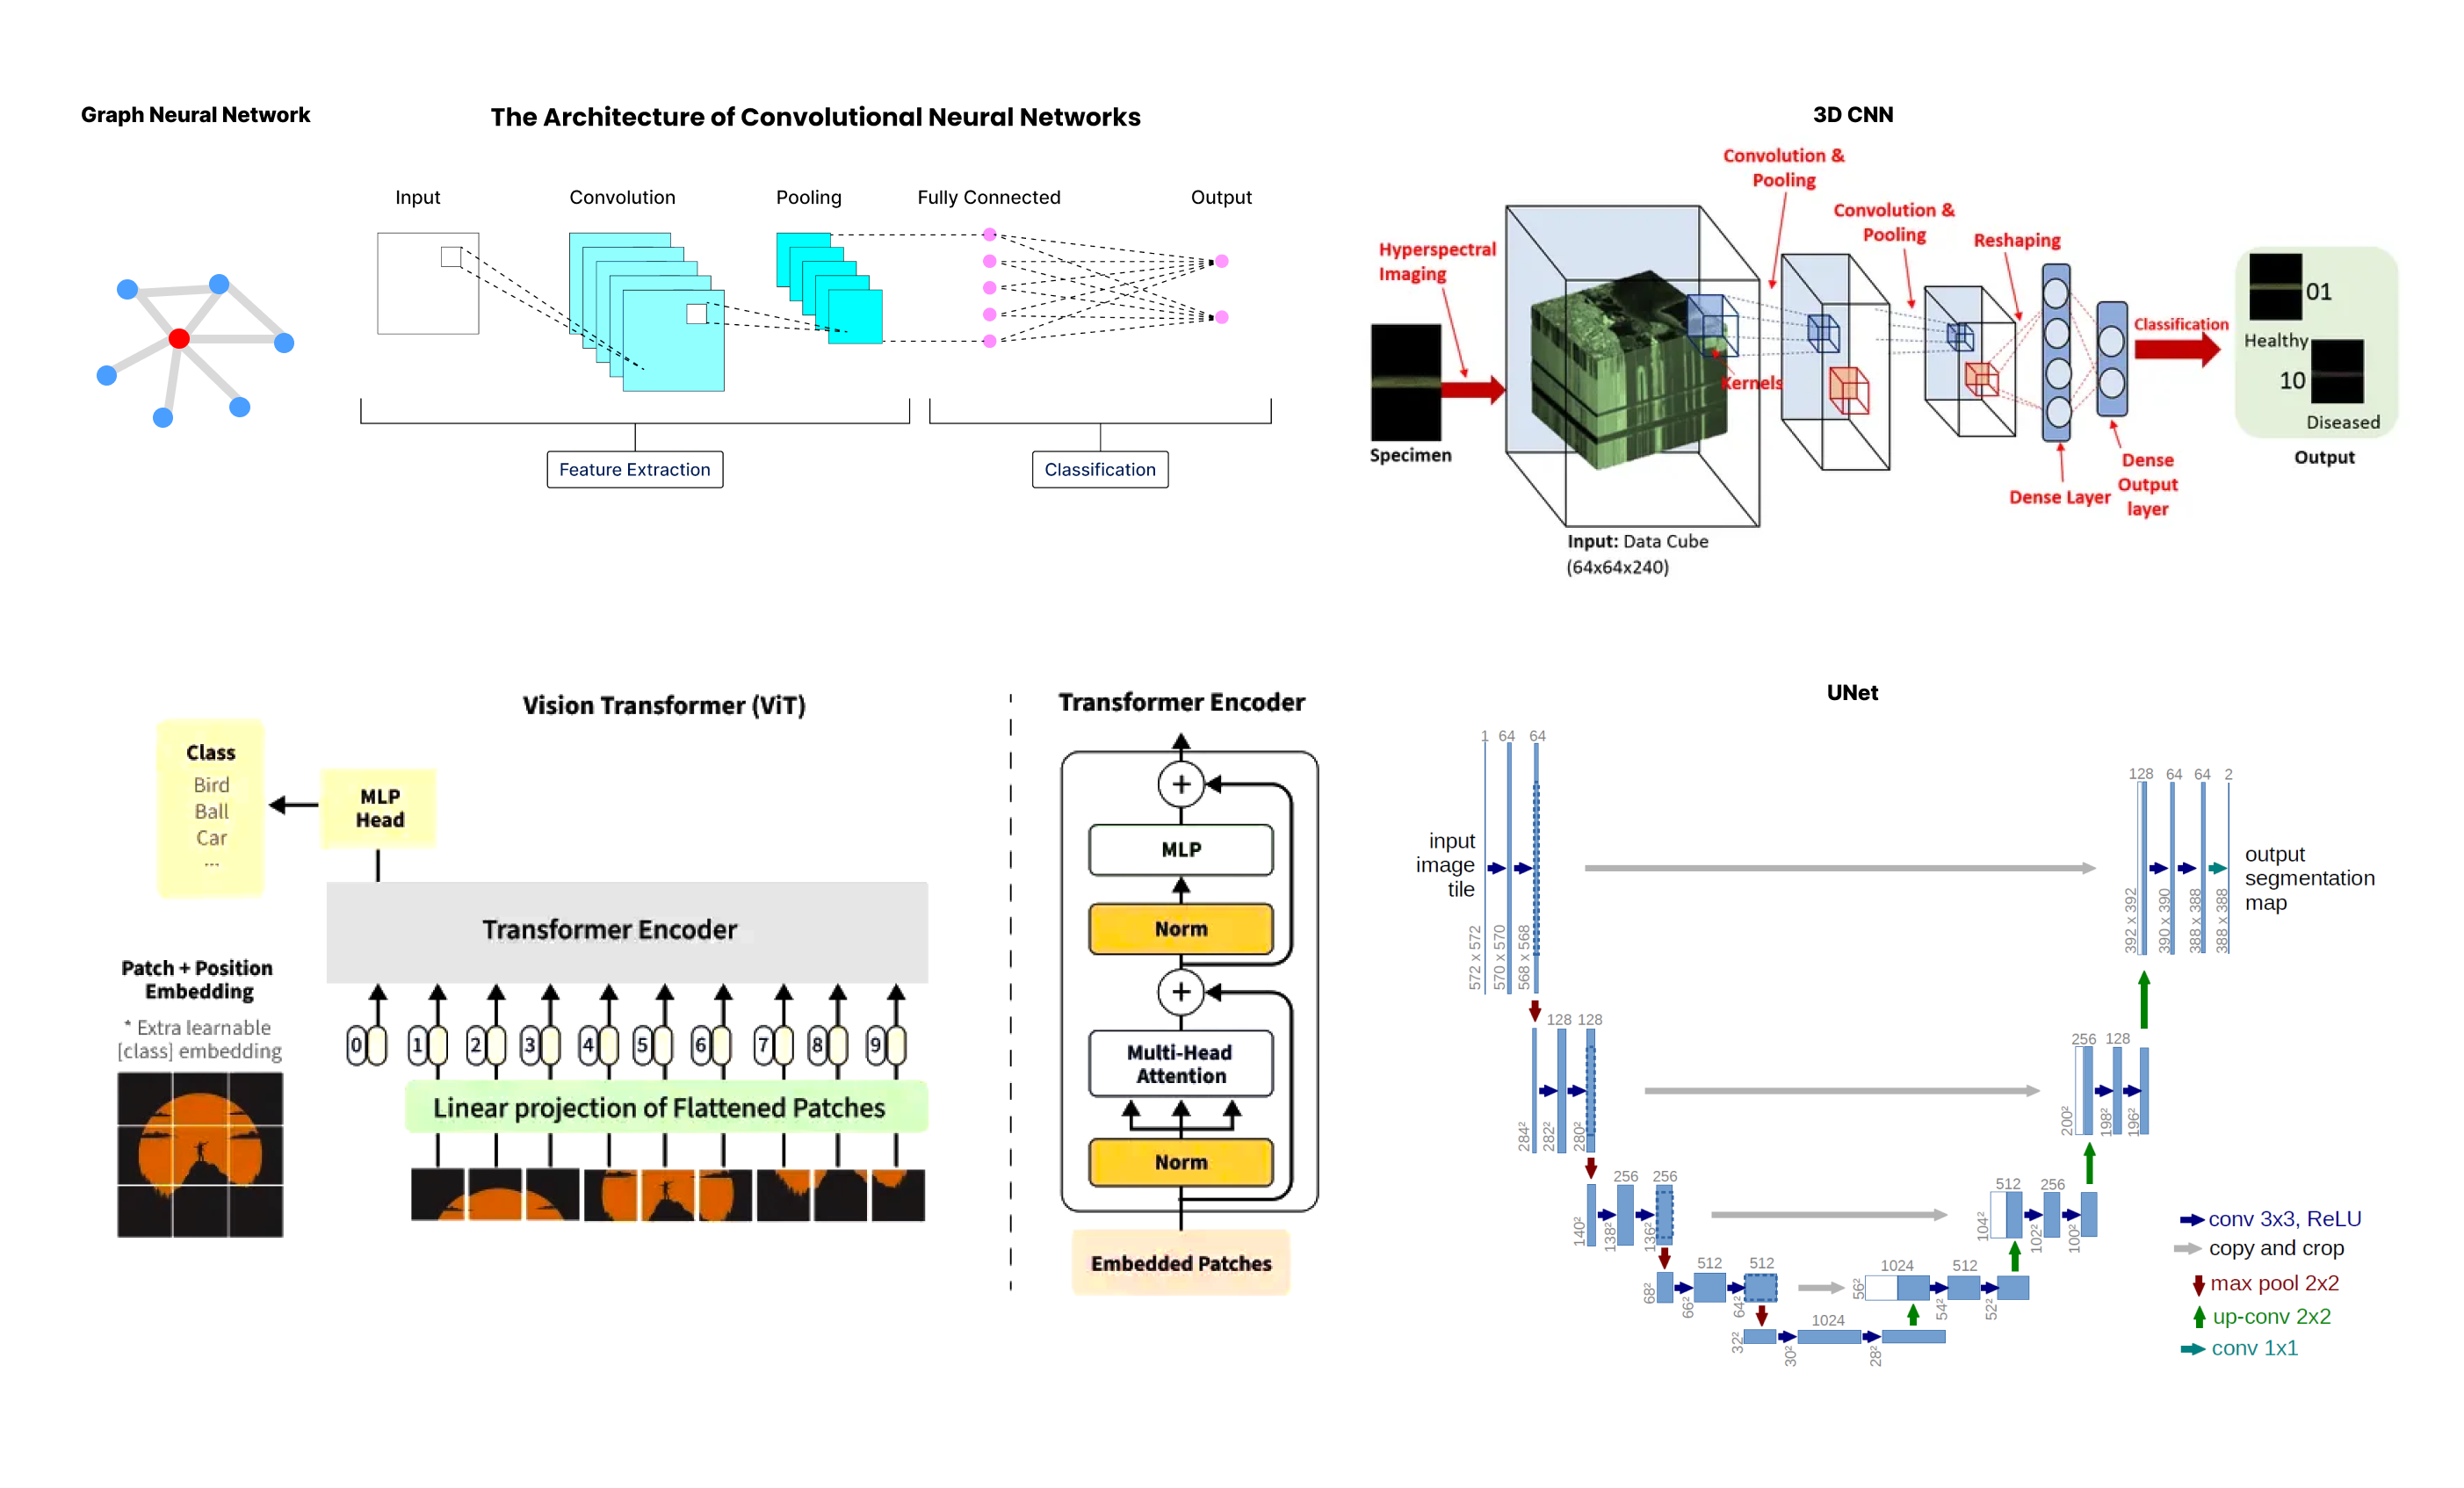
\includegraphics[width=\linewidth]{Spatio.png}
%     \caption{Spatial Model}
%     \Description{An illustration of a spatial model highlighting spatial correlations (e.g., location-based influences).}

%     \label{Spatial Model}
% \end{figure}

\paragraph{Longitudinal modeling}: Longitudinal data require both within subject correlation and between subject variability. The linear mixed-effects model (LMM) separates a fixed effect trend from random per individual intercepts and slopes but assumes linearity; the generalized additive mixed model (GAMM) adds spline based nonlinear trends at the cost of manual basis and smoothness selection. A deep generalized additive mixed model replaces splines with a neural network,
\[
Y_{ij} = \mathrm{DNN}(X_{ij}) + Z_{ij} u_i + \epsilon_{ij},
\]
learning nonlinearities automatically while retaining random effects $Z_{ij}u_i$, though it still struggles with long term dependencies.

Transformer based longitudinal models further add global temporal attention and personalized feature attention, capturing long range dependencies and individual dynamics without manual random effect or spline specification. This progression---from linear and additive mixed models to neural additive and transformer based formulations---successively removes linearity and manual feature constraints, improving personalized longitudinal health prediction.


\section{Spatiotemporal Models in Digital Health}
\label{sec:models}
We now examine four representative digital health domains from the past five years---dietary interventions, diabetes management, depression diagnosis, and cardiac disease---spanning video behavior recognition, regularly sampled time series, brain functional connectivity, and 3D/4D cardiac imaging. For each we summarize the data forms, typical tasks, and representative architectures, and contrast deep spatiotemporal models with classical baselines to surface recurring tradeoffs; Table~\ref{tab:evidence} collects the datasets, metrics, and reported performance of the studies discussed here and in Section~\ref{sec:categorization}.

\subsection{Dietary Interventions}
Dietary data appear mainly as image sequences of eating or exercise behavior, or wearable sensor series rendered as video or raster tensors~\cite{Rouast2020IntakeGesture,Kyritsis2019EatingBehavior}. Tasks center on detecting and classifying eating behaviors and anomalies, often fused with wearable signals (heart rate, activity) for prediction or recommendation. Architectures are typically 2D-CNN plus RNN (LSTM/GRU), or 3D-CNN and ConvLSTM that convolve directly over space and time~\cite{Rouast2020IntakeGesture}. Relative to handcrafted dietary logging, these models detect subtle eating actions automatically and enable individualized intervention, but at the cost of heavy labeling and computation; robustness to lighting, occlusion, and individual variation, along with cross-population generalization, remains the main obstacle, motivating self-supervised or few-shot learning and on-device inference.

\subsection{Diabetes Management and Prediction}
Diabetes data are mostly regularly sampled series---continuous glucose monitor (CGM) readings and regional prevalence rates---with individual trajectory or point reference samples from wearables and EHRs. Tasks include short term glucose forecasting and anomaly alerts, regional incidence prediction for public health, and imputation or insulin dosing. Personal glucose series are modeled with RNN, LSTM, GRU, or Transformers, as in GluNet and related deep forecasters~\cite{Li2020GluNet,Lim2025VirtualCGM}, while regional data use GCNs with temporal modules such as STGCN over geographic adjacency, and spatiotemporal analyses map prevalence across regions~\cite{XiaoLi2016DiabetesSpatiotemporal}; patient specific management is increasingly framed as a predictive digital twin~\cite{Faruqui2024}. Compared with classical statistical glucose models, deep spatiotemporal models better capture nonlinear, multi-scale temporal dynamics but demand more data and offer less interpretability; multi-source heterogeneous fusion and privacy remain the key obstacles, motivating large multimodal datasets and federated learning.

\subsection{Depression Diagnosis and Intervention}
Depression studies use fMRI sequences and EEG series~\cite{2,4}, population counts as raster data~\cite{3}, and dynamic functional connectivity graphs~\cite{4,9}. Tasks span classification, anomaly detection, signal imputation, case forecasting~\cite{3}, and treatment response prediction~\cite{4}. fMRI uses 3D-CNN, ConvLSTM, or ConvLSTM U-Net~\cite{9}; EEG uses CNN plus GRU/LSTM~\cite{2}; dynamic connectivity uses GCN with RNN (STGCN) or attention~\cite{4}. The defining challenge is high dimensional yet small sample data with cross-center heterogeneity: such models capture complex neural dynamics but overfit easily and transfer poorly across sites, motivating self-supervised learning, multimodal fusion, and federated training~\cite{9}.

\subsection{Cardiac Diseases}
Cardiac work uses imaging sequences (MRI, CT, echocardiography) and ECG or intracardiac signals~\cite{5,6,7}. Cine-MRI and ultrasound are video data for segmentation and detection, while ECG signals map onto spatial nodes as raster data or graphs~\cite{7}. Tasks include segmentation, classification (arrhythmia, heart failure), risk prediction, and physics-informed conduction modeling~\cite{7}. Models use 3D-CNN and ConvLSTM (including ConvLSTM U-Net), LSTMs or Transformers for signals~\cite{5,6}, and GNNs or physics-informed networks for electrophysiology~\cite{7}. Embedding physical priors improves accuracy and interpretability over purely data-driven models, yet center-to-center protocol variation, high imaging resolution, and real-time demands still degrade out-of-domain performance, driving interest in lightweight, interpretable, physics-informed multimodal models~\cite{6}.

\subsection{Cross-Domain Patterns in Spatiotemporal Modeling for Digital Health}
Across these domains, several recurring patterns guide model selection and deployment.

\paragraph{Versatility.} All four domains pair CNN or GCN spatial encoders with temporal modules (LSTM/GRU/Transformer) or STGCN to jointly model space and time across video, raster, and EEG data~\cite{2,3,4,6}, differing mainly in priors---anatomical connectivity for depression~\cite{4}, physical equations for cardiac flow and electrophysiology~\cite{5,7}.

\paragraph{Small samples, high dimensions.} Neuroimaging and 4D cardiac data are high dimensional but small in sample due to cost and ethics, risking overfitting and poor transfer~\cite{4,5,6}; physical priors~\cite{7}, active learning, federated learning, and self-supervised attention to salient regions help~\cite{2,4}.

\paragraph{Multimodal fusion.} Integrating environmental, behavioral, and genetic data with the primary signals yields richer assessments---glucose plus geography for diabetes risk maps~\cite{XiaoLi2016DiabetesSpatiotemporal}, physiological or physical priors for cardiac interpretability~\cite{5,7}. Statistics research reinforces this: convection--diffusion and dynamic deformation models encode physical transport and nonstationary dependence, and disease mapping and spatial SIR emulators link exposure, regional outcomes, and temporal dynamics through Bayesian hierarchies~\cite{liu2022convectionDiffusion,castroMorales2025dynamicDeformation,wang2024respiratoryDiseaseMapping,trostle2024spatialSIR,wikle2023statisticalDeepLearning}.

\paragraph{Deployment and efficiency.} Macro scale regional forecasting must incorporate socioeconomic, transport, and mobility factors, where adjacency uncertainty and noise hamper robustness~\cite{2,3}. Rising data resolution raises compute cost~\cite{5,7}, motivating compression, edge computing, and hardware-software co-design for real-time monitoring.

\paragraph{Explainability and standardization.} Clinical use demands interpretable outputs such as attention maps and salient space-time segments~\cite{2,4}, while inconsistent annotation across centers limits reproducibility~\cite{6}, calling for data governance and benchmarking.

\section{DNN-based Medical Models and Longitudinal Models}
\label{sec:categorization}
Complementing the irregular-time and longitudinal \emph{methods} of Section~\ref{sec:history}, this section reviews clinical \emph{studies} that apply DNN based medical and longitudinal models to two tasks---dynamic prediction and risk stratification. These studies leverage longitudinal data, from multivariate clinical measurements to sequential imaging, using multivariate functional principal component analysis (MFPCA), CNNs, Transformers, and recurrent networks for survival prediction, mortality risk, and personalized care. Table~\ref{tab:evidence} synthesizes representative studies across the four application domains and these longitudinal tasks, with their datasets, evaluation metrics, and reported performance; a recurring theme is that attention based models tend to outperform recurrent and convolutional baselines once follow-up data are dynamically incorporated, though reported gains vary and several studies rely on small or private cohorts.

\begin{table*}[t]
\centering
\caption{Quantitative synthesis of representative spatiotemporal deep learning studies in digital health. Values are as reported by the cited studies; \emph{n/r} denotes not reported or not applicable. No quantitative dietary/lifestyle study met our inclusion criteria, consistent with lifestyle factors remaining underused.}
\label{tab:evidence}
\scriptsize
\setlength{\tabcolsep}{3pt}
\renewcommand{\arraystretch}{1.15}
\begin{tabularx}{\textwidth}{>{\raggedright\arraybackslash}p{1.7cm} >{\raggedright\arraybackslash}p{1.5cm} >{\raggedright\arraybackslash}p{2.9cm} >{\raggedright\arraybackslash}p{2.6cm} >{\raggedright\arraybackslash}X >{\raggedright\arraybackslash}p{2.5cm}}
\toprule
\textbf{Study} & \textbf{Domain} & \textbf{Dataset ($n$; access)} & \textbf{Model} & \textbf{Task; reported performance} & \textbf{Baselines outperformed} \\
\midrule
Liu et al.~\cite{2} & Depression, EEG & MODMA, 53 subjects; public & CNN$+$GRU brain-map & Classification; accuracy 89.6\%, F1 90.2\% & SVM, TCN \\
\addlinespace[1pt]
Thaipisutikul et al.~\cite{3} & Depression, population & Thai national, 70 months; public & Multivariate CNN (MONDEP) & Forecasting; MAE 449.7, RMSE 528.1 & SARIMAX, LSTM, TS-Transformer \\
\addlinespace[1pt]
Kong et al.~\cite{4} & Depression, fMRI & 2 hospital cohorts, $\sim$277; private & Spatio-temporal GCN & Diagnosis acc.\ 84.1\%; treatment response 89.6\% & SVM, RF, GCN \\
\addlinespace[1pt]
Bohoran et al.~\cite{5} & Cardiac, CMR & 424 scans / 376 patients; private & Pruned BConvLSTM U-Net & Aortic segmentation; Dice 0.989/0.991 & Bai et al.\ (2018) \\
\addlinespace[1pt]
Xie \& Yao~\cite{7} & Cardiac, EP & Simulation; synthetic & Physics-constrained deep active learning & Wave reconstruction; rel.\ error $\downarrow$ up to 48\% & Spatiotemporal GP \\
\addlinespace[1pt]
Zhang et al.~\cite{9} & Depression, fMRI & OpenNeuro DS002748, 72; public & STANet (CNN$+$RNN, AFGRU) & Classification; accuracy 82.4\%, AUC 90.7\% & SVM, LSTM, Conv-GRU \\
\addlinespace[1pt]
Li et al.~\cite{Li2020GluNet} & Diabetes, CGM & UVA/Padova sim.\ (10) $+$ clinical; mixed & Dilated CNN (GluNet) & 30/60-min forecast; RMSE 8.9/19.9 mg/dL (sim.) & SVR, ARX, NNPG \\
\addlinespace[1pt]
Lim et al.~\cite{Lim2025VirtualCGM} & Diabetes, life-log & 171 adults; n/r & BiLSTM $+$ dual attention & Glucose inference; RMSE 19.5 mg/dL & n/r \\
\addlinespace[1pt]
Li et al.~\cite{XiaoLi2016DiabetesSpatiotemporal} & Diabetes, spatial epi.\ & BRFSS $+$ ACS, 48 states; public & Bayesian spatiotemporal (STAR) & Prevalence mapping; 8.7\%$\to$11.2\% (2004--11) & n/r (epidemiological) \\
\addlinespace[1pt]
Lin \& Luo~\cite{lin2022deep} & Longitudinal, survival & ADNI 1068 $+$ NACC 5261; public & TransformerJM & Dynamic survival; iAUC 0.89/0.81, best calibration & MFPCA-Cox, MATCH-net (mixed) \\
\addlinespace[1pt]
Nitski et al.~\cite{nitski2021long} & Longitudinal, mortality & SRTR 42{,}146 $+$ UHN 3269; registry & Transformer & 1/5-yr mortality; AUROC 0.80/0.73 & MLP, RNN, TCN, LR \\
\addlinespace[1pt]
Glaser et al.~\cite{glaser2022deep} & Longitudinal, imaging & Health ABC, $>$15k scans; public & DenseNet $+$ RNN & All-cause mortality; AUROC 0.79 & Single-scan models \\
\bottomrule
\end{tabularx}
\end{table*}

\subsection{Deep Learning for Dynamic Prediction of Multivariate Longitudinal and Survival Data}
Lin et al.~\cite{lin2022deep} jointly model multivariate longitudinal data and time-to-event outcomes, avoiding the restrictive assumptions of classical joint models. They compare MFPCA based survival models (MFPCA-Cox, MFPCA-DeepSurv), efficient but limited in nonlinear interactions; MATCH-net, a CNN handling irregular sampling and missingness but predicting survival without forecasting trajectories; and TransformerJM, which treats each visit as a token and uses masked self-attention to jointly predict future measurements and update survival probabilities, excelling under nonlinear interactions and non-proportional hazards.

\subsection{Deep Learning Approaches for Long-Term Mortality Risk Stratification in Liver Transplant Recipients}

Nitski et al.~\cite{nitski2021long} forecast 1-year and 5-year mortality in liver transplant recipients from longitudinal clinical data, replacing static logistic regression that ignores follow-up dynamics. Among multilayer perceptron (MLP), RNN, temporal convolutional network (TCN), and Transformer architectures, the Transformer achieved the highest area under the ROC curve (AUROC); trained on the Scientific Registry of Transplant Recipients (SRTR) and externally validated on University Health Network (UHN) data with transfer learning, it enables continually updated, real-time risk stratification.


\subsection{Deep Learning for All-Cause Mortality Prediction from Longitudinal DXA Imaging}

Glaser et al.~\cite{glaser2022deep} predict all-cause mortality from longitudinal total-body dual-energy X-ray absorptiometry (DXA) imaging, showing that deep networks extract predictive features directly from raw scans (alone or with clinical risk factors) and that sequence models over multiple scans outperform single-scan models. They use single-record models (a DenseNet121 over image crops, a fully connected network over clinical metadata, and a combined-modality fusion) and sequence models that feed per visit embeddings to an LSTM to capture the temporal evolution of body composition.


\section{Spatiotemporal Models in Medical Digital Twins}
\label{sec:DT}
Bringing spatiotemporal models into clinical workflows faces three constraints along the symptom--visit--diagnosis--treatment--rehabilitation pathway: (1) insufficient and heterogeneous data, since reliance on recall and self-report creates gaps and inconsistent time labels while constitution, lifestyle, and environment add heterogeneity that no single variable explains; (2) data security and privacy, balancing the use of highly sensitive health information against compliance requirements; and (3) presentation and interpretation, communicating outputs to clinicians and patients across diverse, interdependent data types.

Digital twins address these jointly by building a virtual ``human mirror'' linked to the individual in near real time, aggregating and governing multisource time series from wearables and fixed medical devices with cloud based standardization, temporal alignment, and cross-modal fusion. Population scale longitudinal data improve predictive accuracy and generalization; federated learning enables training under data remain in place constraints; and multidimensional visualization with human in the loop mechanisms present predictions interpretably, closing the loop between decision support and self-management. We next discuss data acquisition and fusion, privacy preserving modeling, and clinical visualization.

\subsection{Digital Twin in Digital Health}

A digital twin (DT) is a cyber-physical feedback loop in which real-time multimodal data from sensors and IoT devices stream to a high fidelity virtual replica, are analyzed, and feed back to the physical asset. Originating in aerospace and manufacturing for full life cycle support~\cite{Tao2018}, in healthcare it emphasizes runtime, with four tiers---visualization and monitoring, prediction, optimization, and closed loop control~\cite{NIST2021,sun2023digitaltwin}. Early work formalized the healthcare digital twin as a virtual patient built from biological and omics data, promising precision medicine while raising ethical questions~\cite{Bruynseels2018DigitalTwins}; at the tissue scale, cell atlas efforts such as the NIH Human Biomolecular Atlas Program (HuBMAP), launched in 2018, map the body at cellular resolution to parameterize a digital twin of the healthy human~\cite{HuBMAP2019}. The most advanced form is the personal digital twin~\cite{deKerckhove2021}.

Personal twins fuse continuous glucose monitors, wearables, home IoT, and genomics into patient specific models. Faruqui \emph{et al.}\ applied transfer learning to a neural network and paired it with a clinician guided feedback controller to generate daily, personalized lifestyle recommendations for managing type 2 diabetes; prediction accuracy exceeded eighty percent and produced sustained improvements in HbA1c and weight~\cite{Faruqui2024}. Silfvergren \emph{et al.} built a multi-organ metabolic model that personalises fasting schedules and macronutrient ratios by simulating hepatic glycogen turnover \cite{Silfvergren2022}. For cardiovascular care, continuous PPG and ECG streams injected into cardiac twins detect atrial fibrillation and impending de-compensation, reducing readmissions \cite{Bayoumy2021,Williams2023}. Because personal twins rely on high frequency, privacy sensitive data, they are increasingly paired with federated learning and differential privacy.



\subsection{Challenges in Data Collection and Prediction for Medical Digital Twins}

In the construction of medical digital twins, data collection is both the most fundamental and one of the most challenging stages. The main difficulty arises from the diversity of data sources. In medical contexts, data originate from electronic health records (EHR), medical imaging (CT, MRI, ultrasound), laboratory test results, physiological signals captured by wearable devices, and real-time monitoring data from ICU systems. These different sources exhibit significant disparities in sparsity and sampling rates: for example, EHR records are sparse and infrequent, whereas ICU monitoring devices capture data at millisecond or second-level granularity; imaging data are usually interval based snapshots that fail to fully capture dynamic processes. Such heterogeneity leads to inconsistencies across temporal, spatial, and semantic dimensions, thereby increasing the difficulty of data alignment and integration.

Moreover, there are substantial differences between modalities, such as textual medical records versus imaging data, or structured laboratory indicators versus continuous physiological signals. Addressing the integration of heterogeneous multimodal data remains a key challenge in the implementation of digital twins in healthcare. Previous studies have pointed out that the standardization and fusion of multi-source heterogeneous medical data are prerequisites for achieving accurate digital twins\cite{tao2019digital,reddy2015healthcare}.

Multimodal fusion is central to the prediction stage, since single modality data (e.g., ECG alone) are noise and gap prone; combining physiological signals, laboratory results, and imaging better simulates progression, with cross-modal alignment mitigating sparsity and single-point failures~\cite{baltrusaitis2019multimodal}, and deep multimodal fusion outperforming unimodal models in cardiovascular prediction~\cite{huang2020fusion}.



Patient heterogeneity complicates prediction: variability from demographics, genetics, environment, disease subtypes, and individual trajectories means identical indicators (e.g., the same BMI or blood pressure) can imply different risks across populations, and ignoring it introduces systematic bias~\cite{obermeyer2016predicting,rajkomar2019machine,yu2018artificial}. Incorporating individual priors---baseline characteristics, genetics, history---into patient specific twins, with Bayesian or meta learning for fast adaptation from little data, improves specificity and robustness~\cite{bjornsson2020digitaltwins}.

Heterogeneity also harms interpretability: complex decision boundaries create a black box effect that undermines clinical trust~\cite{rudin2019stopexplaining}. Since interpretability is as important as accuracy in high risk care~\cite{tonekaboni2019clinicians,lundberg2017unified,voigt2021digital}, twins increasingly use attention based feature attribution, post hoc explanations (SHAP, LIME), and causality driven models with medical knowledge graphs~\cite{ahmad2018interpretable}.

\subsection{Medical Data Privacy Problem and Federated Learning in Digital Twin}

\textbf{Why medical data privacy is critical.} Healthcare data are highly sensitive and valuable on the black market, making the sector a frequent target of identity theft, fraud, and ransomware; a single healthcare breach costs on average about USD 10.1 million, and the 2015 Anthem breach alone exposed nearly 80 million records~\cite{Seh2020HealthcareDataBreaches,Argaw2020HospitalCybersecurity,Nemec2024HealthcareSecurity}. Centralized storage is especially vulnerable, motivating privacy enhancing methods such as blockchain, differential privacy, and federated learning as secure alternatives~\cite{rieke2020digitalhealth,dhiman2022FL}.\begin{figure*}[t] \centering 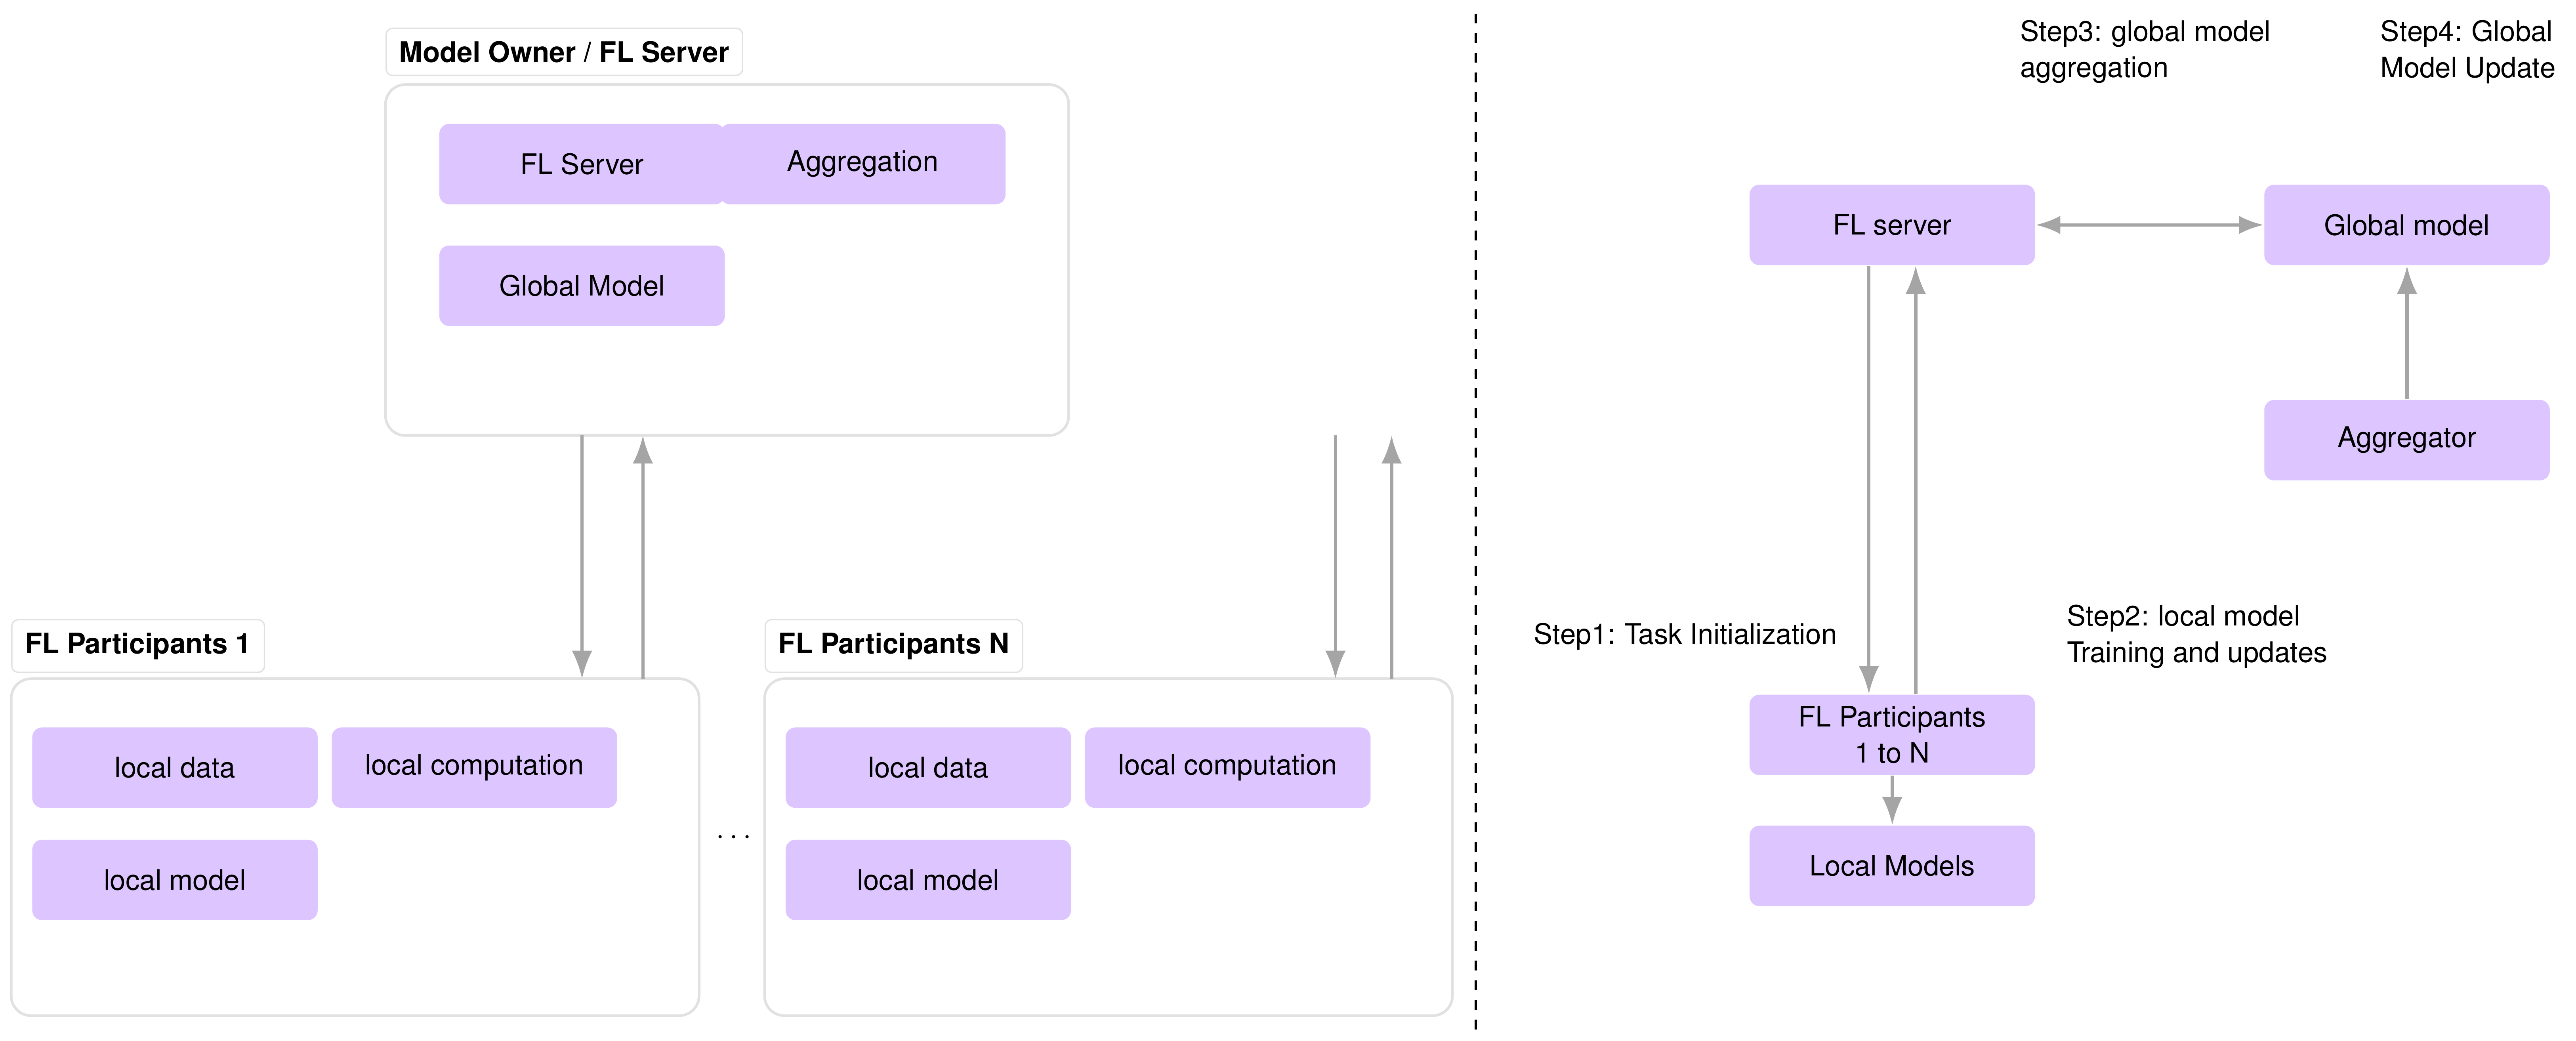
\includegraphics[width=\linewidth]{Fig5_redrawn_600dpi.png} \caption{The federated learning training cycle: a global model is distributed to participating institutions, each trains it locally on its own private data, and only the resulting model updates are returned to a central server for aggregation, so raw patient data never leave the institution.} \Description{A schematic of the federated learning process, showing local training on multiple clients and global aggregation of model updates on a central server without sharing raw data.} \label{fig:Federated Learning Process} \end{figure*}

\textbf{How federated learning works.} FL trains a shared model across institutions without moving raw data (Figure~\ref{fig:Federated Learning Process}): a global model is initialized and sent to clients, each trains locally and returns only encrypted updates, which are aggregated and redistributed iteratively, aiding HIPAA and GDPR compliance. Challenges include communication overhead, non-IID data, and adversarial robustness~\cite{prayitno2021FLhealthcare,coelho2023FLsecurity}.


\textbf{Federated learning for spatiotemporal models in digital twins.} Combining FL with spatiotemporal longitudinal models inside a digital twin yields a privacy preserving pipeline: local twins on edge or hospital servers encode multivariate trajectories (diet logs, CGM traces, regional lifestyle factors) into latent representations, refine a shared network on private cohorts, and send only encrypted updates to an aggregator that synchronizes thousands of twins in compliance with data protection rules~\cite{aouedi2022FLmedical} (Fig.~\ref{fig:architecture of FL}). This enhances personalized optimization and real-time monitoring while letting each twin learn from a larger virtual cohort, valuable in nutrition centric applications where dietary patterns vary by geography yet privacy rules block sharing~\cite{nguyen2022FLsmarthealthcare}. A twin aware stack adds a semantic alignment layer harmonizing site schemas and a feedback layer streaming uncertainties to bedside dashboards; with transformer based encoders, such designs aim to lower glycemic prediction error while reducing communication overhead, though quantitative evidence remains preliminary.

\textbf{Outlook.} Converging edge--cloud FL, explainable spatiotemporal models, and physics informed organ simulators could push digital twins toward closed loop companions that propose, simulate, and verify lifestyle or medication changes before any real action, requiring standardized ontologies, differential privacy for gradient sharing, and lightweight continual learning on wearable class hardware. \begin{figure*}[t] \centering 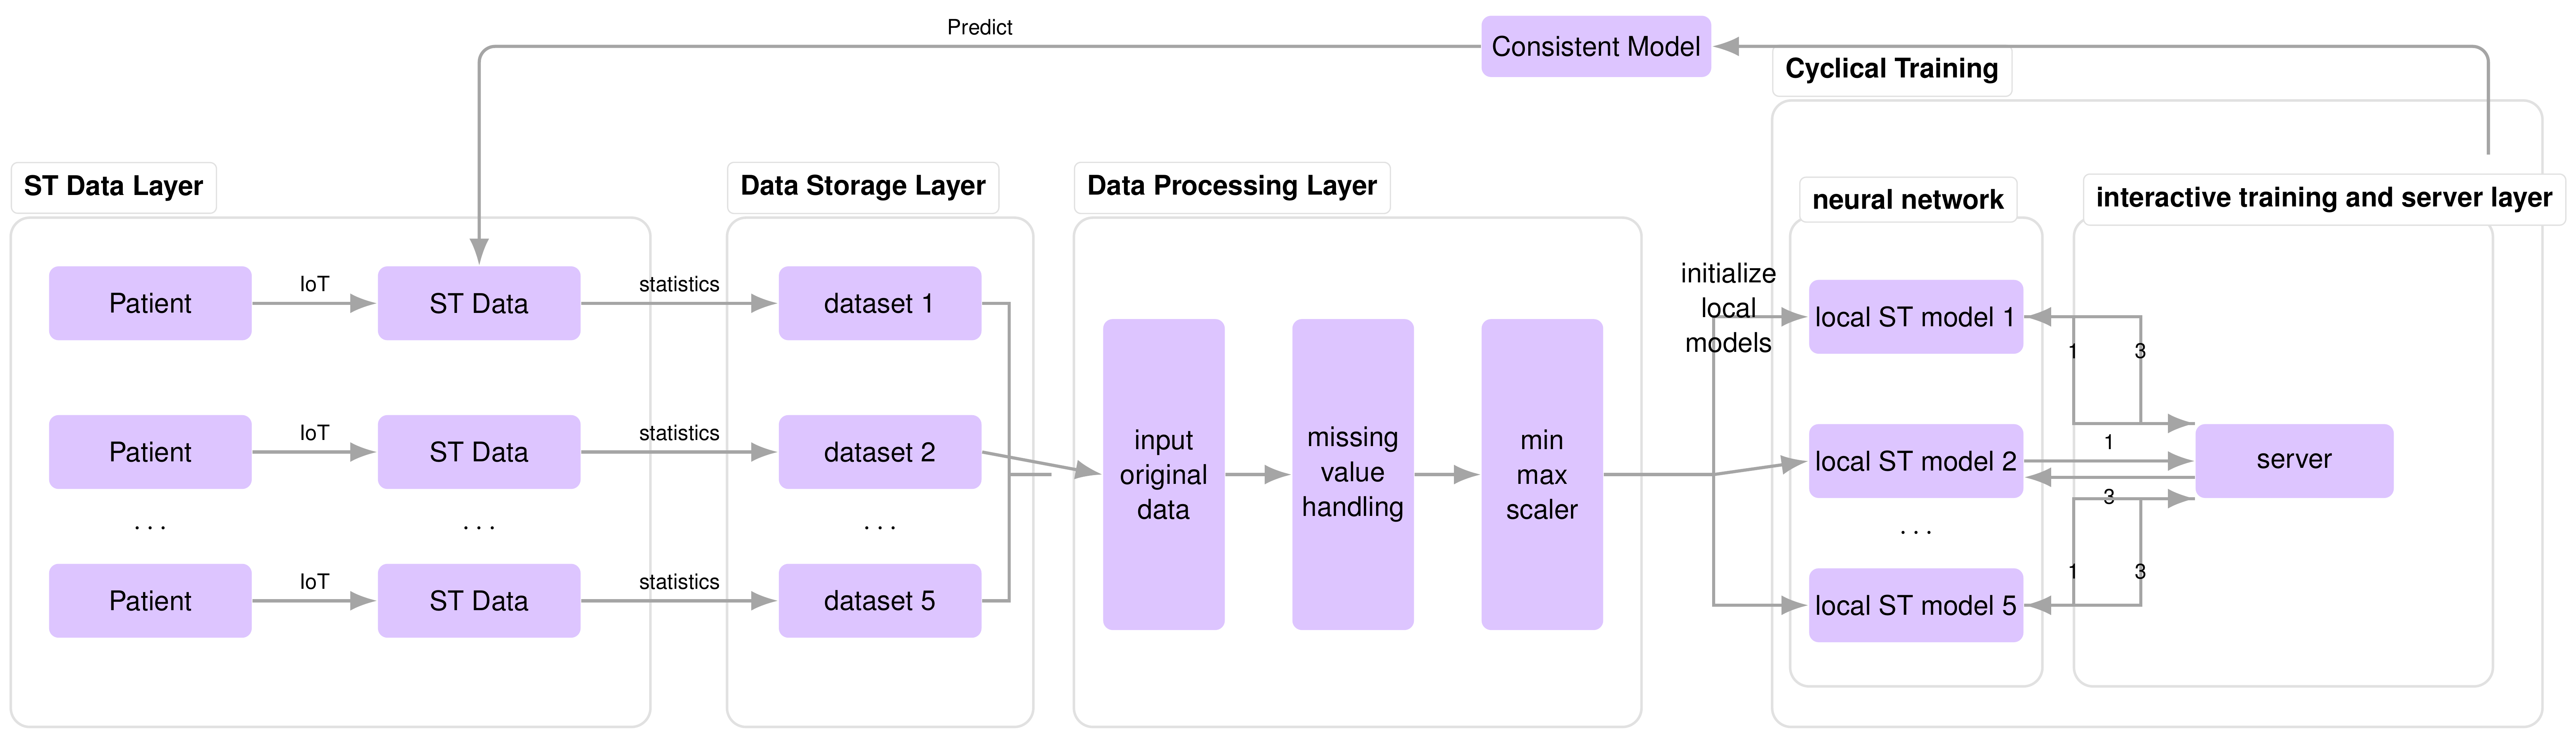
\includegraphics[width=\linewidth]{Fig6_redrawn_600dpi.png} \caption{A general architecture for federated learning of spatiotemporal models in digital health: distributed institutions encode local spatiotemporal patient data, train a shared model on their private cohorts, and exchange only encrypted updates with a central aggregator that synchronizes the per-patient digital twins.} \Description{A general architecture of federated learning for spatiotemporal models in digital health, showing distributed data sources and collaborative training without sharing raw data.} \label{fig:architecture of FL} \end{figure*}
\subsection{Visualization in Digital Twin}

Digital twins enable dynamic, personalized visualization. In surgery, computer generated vitals on a feedback screen improve ergonomics~\cite{Auvinet2018AR}, and with extended reality they overlay operative regions and incision lines for precise cuts~\cite{QUESADAOLARTE20221580}. AI powered twins generate live, data driven graphical analysis for the operating room and routine check-ups~\cite{Vallee2023DT}, while AR display of CT scans supports preplanning~\cite{Southworth2020XR}; preoperative 3D mapping with marked incisions has been shown to shorten surgery time~\cite{Auvinet2018AR}.

For patients, xR presentations aid comprehension: virtual brain models for doctor--patient communication raised satisfaction about 25\% above the average of the HCAHPS standardized patient-experience survey across 257 patients~\cite{Louis2021VR}.

Twins also visualize dietary health over time; Gkouskou et al.~\cite{gkouskou2020virtual} propose lifelong nutritional snapshots integrating metabolomic, immune, behavioral, and gut microbial parameters, feeding a longitudinal spatiotemporal model of nutritional health.

\section{World Model Based Digital Twins in Digital Health}
\label{sec:world_model_dt}
World model based digital twins are a more active form of patient centered twin. Whereas a conventional spatiotemporal model maps history to future outcomes, a world model learns a compact latent state and a transition that can be rolled forward under hypothetical actions. Synchronized with a digital twin, it compresses multimodal observations (EHR, wearables, imaging, mobility, exposures, lifestyle) into an evolving patient state and estimates trajectories under alternative interventions, bridging representation learning, personalized twins, and decision planning~\cite{Zheng2026DTtoWM}.

\subsection{Patient-State Simulation and Counterfactual Planning}
A health world model simulates patient-state evolution rather than predicting a single endpoint: given the current latent state and an action (medication change, diet, rehabilitation, sleep, exposure reduction), it produces a short or long horizon trajectory of physiological, behavioral, or clinical variables. This counterfactual capability is valuable in chronic disease management, where clinicians compare intervention paths before choosing.

Unlike generic generative models, these twins stay anchored to a specific patient: the twin supplies continual synchronization as new observations update the latent state and constrain rollouts, while spatiotemporal learning supplies the representation backbone encoding temporal dynamics and spatial context (regional exposures, organ imaging, mobility, behavior). Together they move from passive monitoring toward active scenario testing, with clinicians retaining final interpretation.

\subsection{Layered Architecture for Spatiotemporal World Models}
An integrated architecture has three layers: spatiotemporal representation models that embed multimodal longitudinal data (physiological series, mobility, imaging, diet, exposures); a digital twin layer maintaining synchronization through continual updating and patient calibration; and a world model layer generating action conditioned rollouts on the twin's latent state, extending the twin from monitoring into simulation and planning with human in the loop review~\cite{Sadee2025MedicalDT}.

This structure shows world models are not isolated modules: their reliability depends on upstream multimodal fusion, temporal alignment, missing data handling, and personalization, and their usability on downstream interfaces conveying assumptions, trajectories, and uncertainty. A world model based twin should thus be evaluated as a coupled system spanning ingestion, representation, simulation, uncertainty, visualization, and workflow integration.

\subsection{Verification, Validation, and Uncertainty}
Verification, validation, and uncertainty quantification are critical because simulated trajectories can influence real decisions. Verification checks that the implementation behaves as intended: pipelines preserve temporal order, action labels map to meaningful interventions, constraints prevent impossible states, and rollouts are reproducible, with stress tests for missing values, delayed or corrupted streams, and distribution shift across sites.

Validation checks clinical credibility. Retrospective comparison with held-out histories is insufficient because most interventions are counterfactual, so validation should add calibration across horizons, subgroup analysis, comparison with mechanistic knowledge, external cohorts, and prospective studies, assessing whether the model ranks interventions consistently with evidence, flags unsafe trajectories, and stays stable under input perturbations.

Uncertainty grows over long rollouts through error accumulation, hidden confounding, partial observability, and multiple plausible futures. A useful system reports calibrated intervals, separates aleatoric from epistemic uncertainty, detects out-of-distribution states, and signals when no reliable recommendation is possible---safeguards essential for trusted decision support rather than opaque simulators~\cite{Sel2025VVUQ}.


\section{Future Prospects of Digital Twin with Spatiotemporal Models in Digital Health Field}
\label{sec:future}
As DNNs advance, spatiotemporal modeling will increasingly integrate multimodal sources, improve efficiency through parallel computing, enhance interpretability, and adopt secure learning. We outline key directions below.
\paragraph{The Value of Digital Twin and Spatiotemporal Modeling in Digital Health}

Healthcare faces fragmented data, delayed diagnosis, limited personalization, and inefficient resource use, with scarce continuous high-quality data limiting AI. Digital twins with spatiotemporal modeling address this by maintaining real-time virtual patient representations updated from wearables, records, environmental sensors, and mobility, from which spatiotemporal models simulate trends, forecast progression, and support decisions while generating high-resolution, temporally aligned data~\cite{ali2024spatialtwins}. Wider adoption should accumulate diverse datasets and enable standardized cross-population models~\cite{bilal2025cityseircast}.

\paragraph{Exploration of Spatiotemporal Models and Technological Advancements}

Across dietary, diabetes, depression, and cardiac applications, deep learning consistently captures spatiotemporal dependencies and integrates multimodal information, aided by big data, cloud, and parallel computing. Key challenges remain: limited data availability and quality, privacy and cross-center collaboration, underexplored multimodal fusion, and real-time and generalization constraints. Privacy preserving methods such as federated learning and differential privacy are therefore essential, and as wearables, self-supervised learning, physics informed constraints, and edge computing mature, clinical adoption will require standardized protocols, robust data protection, reliable models, and tight workflow integration.
\paragraph{Promoting Data Sharing in Digital Health Research}
Digital health integrates heterogeneous data from hospitals, wearables, environmental sensors, and genomics, so standardized collection, annotation, and exchange protocols are essential. Federated learning and secure multi-party computation let institutions retain data autonomy while collaborating, but only joint technical and legal progress can overcome data silos for precise monitoring and intervention.

\paragraph{From Clinical Trials to Real World Commercial Applications}
Translating these technologies to market requires stability and scalability in dynamic settings, balancing accuracy with cost, security, and user experience, and moving from controlled trials to population scale use through collaboration with insurers, pharma, and hospitals, with continuous iteration on user feedback.

\paragraph{Future World Model Based Digital Twins}
Future systems will likely benefit most from constrained world models synchronized through digital twins and informed by spatiotemporal context, compressing multimodal data into latent health states, updating continually, and rolling forward under candidate interventions. The challenge is combining the adaptability of world models with the personalization, synchronization, and accountability of medical twins, requiring hybrid mechanistic learning, multiscale organ--person--environment representations, privacy preserving continual learning, and prospective validation before deployment~\cite{DeDomenico2025ComplexSystems}.
\bibliographystyle{IEEEtran}
\bibliography{newST}
\end{document}

\endinput
%%
%% End of file `sample-acmcp.tex'.
